\documentclass[english,aps]{article}
\usepackage[T1]{fontenc}
\usepackage{amsmath}
\usepackage{graphicx}
\usepackage{amssymb}
\usepackage{float}
\usepackage{alltt}
\usepackage[margin=1in]{geometry}
\usepackage{longtable}
\usepackage{multirow}
\usepackage[colorlinks]{hyperref}
\makeatletter
\usepackage{babel}
\makeatother
%\pagestyle{fancy}
\title{Menard 2016 MFE Concept\\ Proprietary Report} 
\author{S. Woodruff, A. Higginbottom}
\date{\today}
\begin{document}
\maketitle
\maketitle
\begin{figure}[t!] 
\centering 

\includegraphics[scale=0.5]{StandardFigures/WSLTD_logo.png} 
\label{fig:logo} 
\end{figure} 
\begin{figure}[h!] 
\centering 
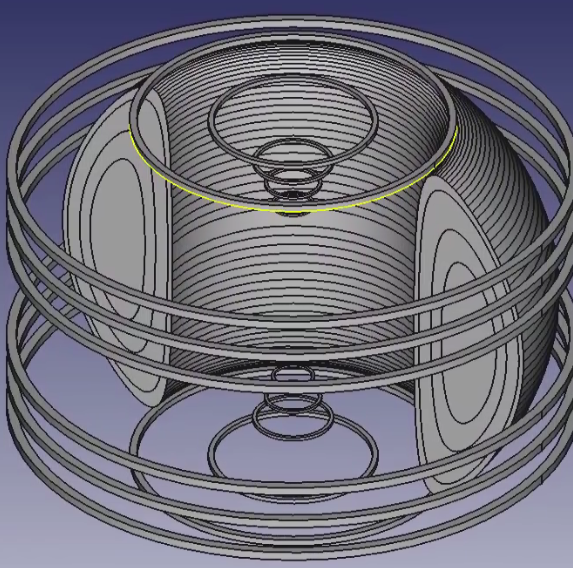
\includegraphics[scale=0.7]{{Figures/MFE.png}} 
\caption{MFE Fusion Energy System} 
\label{fig:render} 
\end{figure} 
\newpage 
\textbf{Foreword} \\ 
 
In the last several years, Woodruff Scientific has maintained an active interest in the costing analysis for fusion energy systems, collaborating with many in the field, and publishing a series of papers on this topic starting in 2011 with basic community consensus on the `Path to Market' for fusion energy systems, outlining the constraints placed on any energy technology as it moves towards commercialization in terms of timeline and available capital, and market demand for smaller, more modular units \cite{Woodruff2012}.  We followed up this analysis with a specific embodiment of a compact modular fusion power core that could be developed privately \cite{Woodruff2015}, working in the context of an IAEA Coordinated Research Project on compact fusion neutron sources and developing a costing model based on the ARIES methodology.  In 2017, we found support from ARPA-E to further develop our costing model in collaboration with Bechtel \cite{Bechtel2017}.  For that costing study, we considered 4 of the concepts that were supported by ARPA-E under the ALPHA program, and worked with PIs in each organization to develop basic radial builds of the 4 fusion power cores, based on prior art, and then performed cost analysis with the Balance of Plant and tritium systems analysis provided by Bechtel, but based predominantly on historical studies.  In 2018 Woodruff organized a workshop for the IAEA on private fusion enterprises \cite{IAEA2018}, and the commercialization path for fusion, with contributions from most major private fusion institutions and provided a summary of the cost modeling underway.\\ 
 
In 2019 ARPA-E revisited the 2017 costing analysis in the light of new costing paradigms developed by Ingersoll and Foss at Lucid Catalyst \cite{MIT2018} \cite{EON2018}, addressing every assumption in the Cost Accounting Structure (CAS), calculating  an updated \$/kW for most CAS outside of the fusion power core (drawing in particular on the DOE NETL report \cite{JamesCorrespondingAuthor2019}). The 2019 ARPA-E study revisited the analysis using the code developed for the four concepts, touching on most of the recommendations of the prior study and obtaining review by leading experts in the field.  The costing was revisited in 2020 to extend to all ARPA-E supported fusion concepts, and the final version was started in 2023 to be released publicly.  This study captures the most recent thinking and brings together all our understanding of best costing methodologies uncovered in the couse of the ARPA-E work.\\ 

\begin{figure}[h!] 
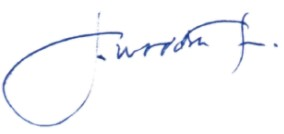
\includegraphics[scale=0.55]{{StandardFigures/signature.jpg}} 
\label{fig:signature} 
\end{figure}


Simon Woodruff \\

President \\

Woodruff Scientific LTD
\newpage
\tableofcontents
\newpage 

\section{Methodology} 

In this cost report, we draw on three major reports that summarize the cost categories for a power plant, based on the methodology developed first by the IAEA, then by the GENIV Economics Modeling Working Group (G4EMWG), and by the lead of the G4EMWG. Geoffrey Rothwell, in his book 'Economics of Nuclear Power'.  There is purposeful use of existing well-documented and contemporary cost basis methodologies represented in these reports, as this documentation will assist anyone who wishes to perform similar analysis.\\

The cost categories depart from prior fusion costing studies by breaking the direct costs into categories 10 (pre-construction) and 20 (construction) and the indirect costs into categories 30-60 (formerly 91-98).  There are some major similarities (in 20, for example, they are almost exactly the same, except for inclusion of a digital twin and contingency), and there are minor variations of the categories that make a lot more sense, for example decommissioning costs are included as a capitalized indirect cost rather than added somewhat obscurely to the LCOE, allowing deeper discussion of the contributing costs to decommissioning.  In this section we describe the main texts that are foundational to the methodology and also those that provide information on cost basis.  Fusion systems of course depart significantly from those of fission in the heat island, fuel cycle, handling, and replacement schedule of major cost components - those are spelled out in each section.  We adopt the subcategory descriptions of most of the GENIV subcategories, but have edited those to more narrowly capture the fusion system costs.\\  

Our philosophy has been to provide recent cost basis information for all cost categories, and state those in the text, providing a reference to the cost basis, and any other reference that will assist the user of the code.  We have also tried to be judicious in our use of terminology: at the time of writing, the term `reactor' is still viewed unfavorably and it's continued use may cause hurdles in the adoption of fusion energy systems, so we have replaced with `heat island'.  For old hands, and those in the nuclear sector, this change in terminology may seem to be superficial, since currently there is renewed interest in nuclear power as a solution for climate mitigation.  We will evolve the terms as necessary, but for this edition, we try to be consistent in the use of terminology that conveys function without connotations.

\begin{figure}[h!] 
\centering 
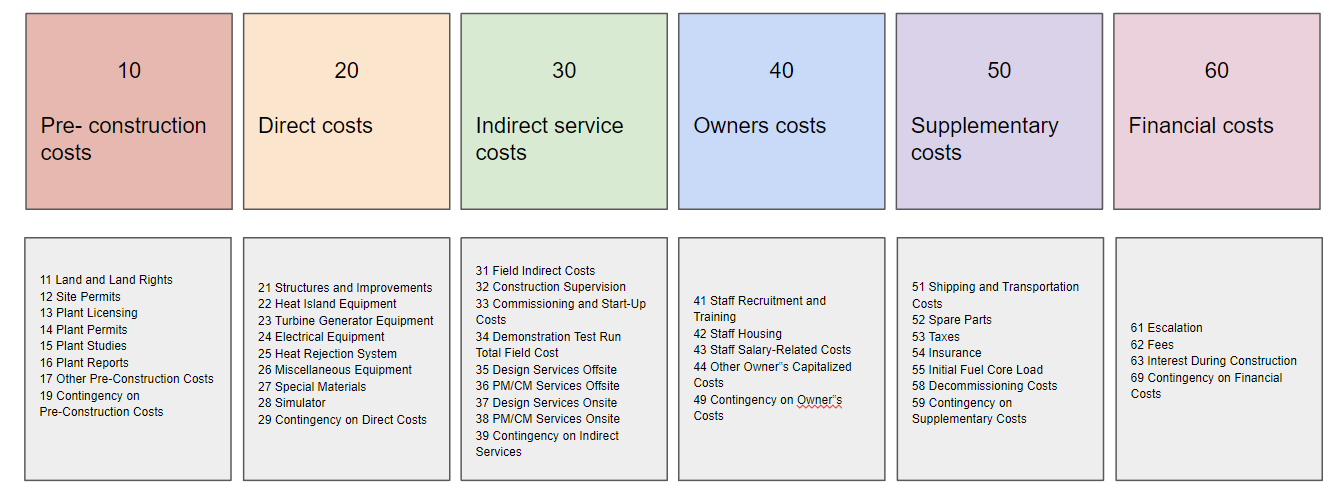
\includegraphics[scale=0.45]{{StandardFigures/costcategories.png}} 
\caption{Cost categories outlined below} 
\label{fig:costcategories} 
\end{figure}

\subsection{Documents influencing the costing methodology}

The GENIV Economics Modeling Working Group (G4EMWG) Guidelines \cite{EMWGOGIIF2007} is a comprehensive guide providing detailed guidelines for economic modeling within the context of Generation IV nuclear energy systems. It systematically outlines the structure for cost estimation, covering various cost categories ranging from pre-construction costs to annualized financial costs. These include detailed breakdowns for capitalized costs (like direct costs, indirect service costs, owner’s costs, and supplementary costs), as well as operational and maintenance costs, fuel costs, and financial costs. The document is meticulously organized, offering a granular view of each cost component, including land rights, permits, licensing, structures, equipment, and contingency costs. It serves as an essential resource for accurately assessing the economic feasibility and overall budgeting for advanced nuclear power plant projects. The guidelines emphasize the importance of detailed cost accounting for ensuring financial viability and strategic planning in the nuclear energy sector.\\

The book "The Economics of Future Nuclear Power", by Geofrey Rothwell \cite{Rothwell2015}, is a comprehensive analysis of the economic factors influencing the future of nuclear power.  The document broadly delves into various aspects such as cost estimation, risk aversion, and capital cost determination for nuclear power projects. It discusses the intricacies of financial modeling and risk assessment, emphasizing the importance of accurately gauging uncertainties and potential costs associated with nuclear energy development. The text also explores the concept of risk diversification, applying financial market theories to the realm of nuclear power investment and development. The content is quite technical, focusing on economic and financial theories as they apply to the nuclear power industry, with detailed mathematical and statistical analyses to support its discussions.\\

The IAEA Tecdoc TRS396 \cite{Meyer2000} is a technical report by the International Atomic Energy Agency (IAEA), providing comprehensive guidelines and methodologies for economic evaluation in the nuclear power sector. The report delves into the economic analysis of nuclear power plants, offering detailed methods for calculating the Levelized Discounted Electricity Generation Costs (LDEGC). It incorporates a range of financial aspects including capital investment costs, operation and maintenance costs, and nuclear fuel cycle costs. The report also discusses the significance of various economic parameters such as discount rates, inflation, and escalation rates in the assessment of nuclear power projects. Additionally, it offers insights into sensitivity analysis, which is crucial for understanding the impact of varying economic conditions on project viability. The document is a valuable resource for professionals in the nuclear industry, providing a structured approach to evaluating the economic feasibility of nuclear power projects.

\subsection{Documents providing cost bases}

The UCSD Report titled "ARIES Cost Account Documentation" by L. M. Waganer, dated June 2013, from the University of California San Diego's Center for Energy Research \cite{Waganer2013}, is a comprehensive documentation of the ARIES Cost Account. Its purpose is to document the historical economic basis for the ARIES Systems Code costing analyses and develop an updated economic model for future systems studies. It provides a thorough background on previous fusion studies' costing information, detailing conceptual designs and cost data from projects like Starfire, Generomak, and various Inertial Fusion Energy (IFE) designs. The report discusses the importance of historical cost escalation, explaining how past estimates are adjusted to current economic conditions using factors like the U.S. GDP Implicit Price Deflator. It also revisits the general cost account information, originally defined by DOE through the Pacific Northwest Laboratory, and covers various aspects such as spare parts, contingency, and Level of Safety Assurance (LSA) in cost estimation. The document offers a detailed analysis of direct and indirect capital costs, elaborating on each cost account with respect to fusion power plants and their respective costing algorithms, adjustments, and recommendations.\\

The presentation titled "Progress On Cost Modeling - Cost Accounts 20 and 21" by L. M. Waganer, dated 14-15 June 2007 \cite{Waganer2007} is centered on the ARIES Project and focuses on improving and updating cost modeling for fusion power plant designs. It discusses the need for revising the ARIES systems code cost modeling, originally based on models from the early 1990s, due to lack of extensive documentation and limited depth in published cost data. The document highlights various cost accounts, like Cryogenic Cooling, Radioactive Waste Treatment, and Reactor Plant Maintenance Equipment, and stresses the necessity for their detailed documentation. The presentation also touches upon general costing ground rules, safety assurance levels, and provides recommendations for defining and reporting cost accounts with reasonable depth. It includes specific details about costs related to land rights, structures, and site facilities for a fusion power plant, proposing updated cost estimates and methodologies for more accurate and comprehensive financial planning in the context of advanced nuclear fusion research.\\

The document "NETL Cost and Performance Baseline for Fossil Energy Plants Volume 1: Bituminous Coal and Natural Gas to Electricity" \cite{JamesCorrespondingAuthor2019} provides an independent assessment of the cost and performance of selected fossil energy power systems. These systems include Integrated Gasification Combined Cycle (IGCC), Pulverized Coal (PC), and Natural Gas Combined Cycle (NGCC) plants. The assessment is conducted using a systematic, transparent technical, and economic approach. This report is the first in a four-volume series, each addressing different aspects of fossil fuel-based power generation. It plays a critical role in assessing and determining technology combinations for future power markets, offering insights for technology comparisons, and providing a framework for regulators and policymakers. In total, nineteen power plant configurations are analyzed, including various IGCC configurations with and without CO2 capture, PC power plant configurations both subcritical and supercritical with varying levels of CO2 capture, and NGCC power plant configurations with state-of-the-art combustion turbines, again with varying levels of CO2 capture.

\subsection{Prior related costing studies}

ARIES, Sheffield, other MFE studies (already in verbose review).



\section{Power balance} 
\begin{figure}[h!] 
\centering 
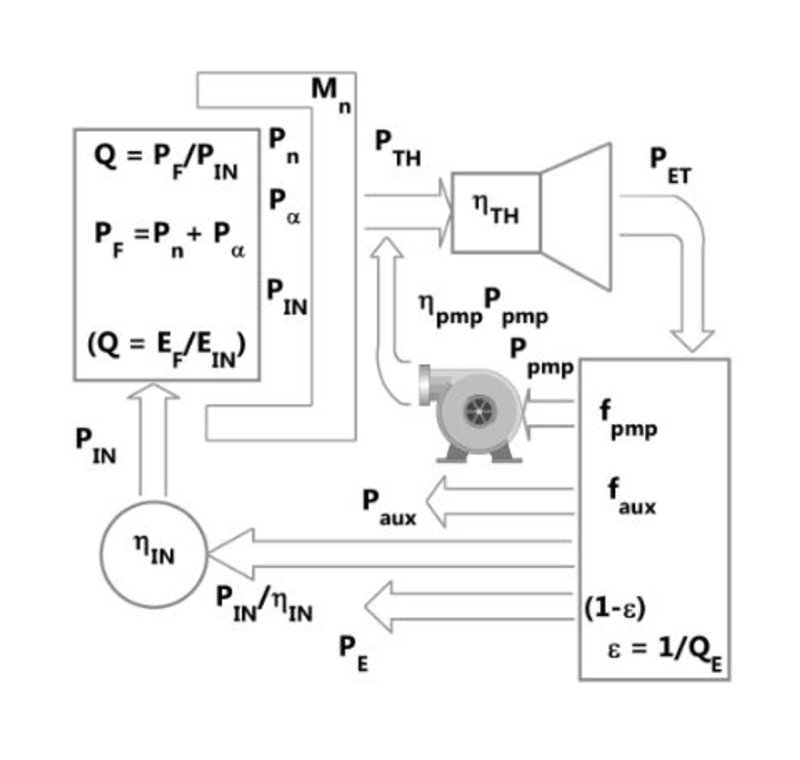
\includegraphics[scale=0.6]{StandardFigures/power.eps} 
\caption{Fusion-based electric power station power-flow diagram.}
\label{fig:pwr} 
\end{figure} 
A representative power-flow diagram for a fusion-based electric power station is presented in Fig. \ref{fig:pwr}. Power, $P_{IN}$, is input to the fusing plasma with efficiency, $\eta_{IN}$. For the D-T fuel cycle, the fusion power, $P_{F}$, is partitioned 20 \% to 3.52-MeV alpha particles and 80 \% to 14.06-MeV neutrons, is relatable to the input power by the gain, Q, as a figure of merit. In a Li-bearing blanket, the neutron power is multiplied by a factor, $M_{n} \simeq 1.1$.  The useful thermal power is $P_{TH}$, which is converted by a turbine-generator (TG) set to a gross electric power, $P_{ET}$.  A fraction of $P_{ET}$ is recirculated to provide $P_{IN}/\eta_{IN}$ as well as pumping power for the primary coolant and other housekeeping power.  The total recirculating power fraction is $\epsilon$, a figure of merit that monitors site power. The net electric power available for sale to the grid is $P_{E} = (1 - \epsilon)P_{ET}$. Not shown on the diagram is the lost power, $P_{Loss} = (1 - \eta_{TH})P_{TH} + (1 - \eta_{IN})P_{IN}/\eta_{IN}$. An alternative definition, $Q_{E} = (1 - \epsilon)/\epsilon$, is sometimes used.  In the desirable limit of low $\epsilon$, these expressions converge asymptotically. Note that the latter form is what was used recently by Wurzel and Hsu \cite{Wurzel2022}. \\

Given a stipulated target for the net electric-power output, $P_E$, the thermal-power output, $P_{TH}$, is determined for a value of the thermal conversion efficiency, $\eta_{TH}$, such that \hbox{$P_E = (1-\epsilon) \eta_{TH} P_{TH}$}, where \hbox{$\epsilon = 1/Q_E$} is the recirculating power fraction and $Q_E$ is the engineering gain.   The gross electric-power output is \hbox{$P_{ET} =\eta_{TH} P_{TH}$}. A fraction $f_{aux}$ of $P_{ET}$ ($P_{aux} = f_{aux} P_{ET}$) is allocated  for auxiliary functions (coolant and housekeeping); a fraction of the gross electric power is allocated to cryo systems, $P_{cryo}$. A fraction  $f_{pump}$ of $P_{ET}$ (\hbox{$P_{pump} = f_{pump} P_{ET}$}) is allocated for primary-loop pumping power. It is assumed that \hbox{$\eta_{pump}  \, P_{pmp}$} is recoverable as useful thermal power in the primary coolant loop.  These fractions of the gross electric power, including also the input power ($P_{IN}$) are commonly referred to as recirculating power. The engineering gain, $Q_E$, can be written as: 


\begin{eqnarray}
\label{e-2-53}
Q_E & = & \frac{1}{\epsilon} \: = \: \frac{P_{ET}}{(P_{ET} - P_{E})}  
\end{eqnarray}
\begin{eqnarray}
\label{e-2-54}
Q_{E} & = & \frac{\eta_{TH}(M_NP_{neutrons}+P_{\alpha}+P_{IN}+ \eta_{pump}P_{pump})}{(P_{aux} + P_{pump}+P_{IN}/\eta_{IN} + P_{cryo} +P_{sub} + P_{control})} 
 \end{eqnarray}
Pending detailed evaluation, the pump efficiency is taken to be $\eta_{pump} = 0.98$, the primary-coolant pumping power is $P_{pump} = f_{pump} \, P_{ET}$, and the auxiliary power is $P_{aux} = f_{aux} \, P_{ET}$, consisting of power to the coolant systems and housekeeping power.
The ratio of fusion power to input power is the fusion gain, \hbox{$Q \equiv P_{F}/P_{IN}$}, where the fusion power is $P_{F} = P_{neutrons} + P_{\alpha}$. Reworking this equation to eliminate explicit powers, the required D-T fusion gain, Q, to achieve a target recirculating power $\epsilon$ derived from the power-flow diagram to be
\begin{eqnarray}
\label{e-2-54}
Q & = & \frac{1}{(0.2 + 0.8 M_n)}
\left[\frac{(1/\eta_{TH} - f_{pump} \,\eta_{pump})(1/\eta_{IN})}{(\epsilon - f_{pump} \,\eta_{pump} - f_{aux})} - 1]\right] \: .
\end{eqnarray} 
The above equation is applicable to most steady-state D-T fusion approaches.  A design-space plot is provided as Fig. 3 of Ref. \cite{Miller2007}. For systems with some recaptured (REC: direct conversion) power, the required gain, Q, becomes: 



\begin{eqnarray} 
\label{e-2-55} 
Q & = & \left[\frac{(1/\eta_{TH} - f_{pump} , \eta_{pump})(1/\eta_{IN} - \eta_{REC})}{(\epsilon - f_{pump} , \eta_{pump} - f_{aux})} - (1 - \eta_{REC}) \right] 
\end{eqnarray}

A design-space plot with $\eta_{REC} = 0.5$ is provided as Fig. 4 of Ref. \cite{Miller2007}. \\

%For a pulsed fusion system, it is convenient to define the plasma internal energy as $W_{IN} = P_{IN}\tau_{d}$, where $tau_{d}$ is the dwell time between fusion pulses.  The fusion energy released per pulse is $W_{F}$ such that the continuous fusion power available to the primary loop is $P_{F} = W_{F}/(\tau_{d} + \tau_{b})$, where $\tau_{b}$ is the pulse (or burn) duration. Expressed in terms of energy, a gain, $Q^{*}$, can be defined as

%\begin{eqnarray} 
%Q^{*} = \frac{W_F}{W_{IN}} = \frac{P_{F}(\tau_{d} + \tau_{b})}{P_{IN}\tau_{d}} = Q(1 + \tau_b/\tau_{d})
%\end{eqnarray}

%A short $\tau_{b}$ implies a large fusion power pulse and $Q^{*}$ approaching Q.
%needs packages \usepackage{graphicx}   \usepackage{float} 
\newpage
\subsection{Power Accounting Table}

\begin{table}[ht!]								
\centering								
\begin{tabular}{|c|p{5cm}|c|c|c|}								
\hline								
\textbf{Account}	&	\textbf{Power Account Description}	&	\textbf{Parameter }	&	\textbf{Power}	&	\textbf{Units} \\
\hline								
1	&	Output power	&		&		&	\\
\hline
1.1	&	Fusion Power	&	$P_{{fusion}}$	&	512	&	MW \\
1.2	&	Alpha Power	&	$P_{{\alpha}}$	&	102.5	&	MW \\
1.3	&	Neutron Power	&	$P_{{neutrons}}$	&	409.5	&	MW \\
1.4	&	Neutron Energy Multiplier	&	$M_N = P_{{TH}}/P_{{fusion}}$	&	1.1	&	\\
1.5	&	$P_{pump}$ capture efficiency	&	$\eta_{{pump}}$	&	0.5	&	\\
1.6	&	Thermal Power	&	$P_{{TH}}$	&	522.7	&	MW \\
1.7	&	Thermal conversion efficiency	&	$\eta_{{TH}}$	&	0.5	&	\\
1.8	&	Total (Gross) Electric Power	&	$P_{{ET}}$	&	235.2	&	MW \\
1.9	&	Lost Power	&	$P_{{Lost}}$	&	287.5	&	MW \\
\hline								
2	&	Recirculating power	&		&		&	\\
\hline
2.1	&	Power into coils 	&	$P_{coils}$ &	5	&	MW \\
2.1.1	&	Power into TF coils	&	$P_{tf}$	&	4	&	MW \\
2.1.2	&	Power into PF coils	&	$P_{pf}$	&	1		&	MW \\
2.2	&	Coolant Pumping Power Fraction	&	$f_{{pump}}$	&	0.1 &	\\
2.2.1	&	Coolant Pumping Power	&	$P_{{pump}} = f_{{pump}} \cdot P_{{ET}}$	&	14.1	&	MW \\
2.3	&	Subsystem and Control Fraction	&	$f_{{sub}}$	&	0.1	&	\\
2.3.1	&	Subsystem and Control Power	&	$P_{{sub}} + P_{{control}} = f_{{sub}} \cdot P_{{ET}}$	&	18.8	&	MW \\
2.4	&	Auxiliary systems	&	$P_{{aux}} = P_{{t}} + P_{{h}}$	&	14.0	&	MW \\
2.4.1	&	Tritium Systems	&	$P_{{t}}$	&	10.0	&	MW \\
2.4.2	&	Housekeeping power	&	$P_{{h}}$	&	4.0	&	MW \\
2.5	&	Cryogenic systems	&	$P_{{cool}} = P_{{TF}_c} + P_{{PF}_c}$	&	2	&	MW \\
2.5.1	&	TF coils cooling	&	$P_{{TF}_c}$	&	1	&	MW \\
2.5.2	&	PF coils cooling	&	$P_{{PF}_c}$	&	1	&	MW \\
2.5.3	&	Cryo vacuum pumping	&	$P_{{p}_c}$	&	0.5	&	MW \\
2.6.	& Input power 	& $P_{IN}$	&	501	&	MW \\
2.6.1	& Input power wall plug efficiency  &	$\eta_{IN}$ & 11	&	MW \\
\hline								
3	&	Output power	&		&		&	\\
\hline
3.1	&	Scientific Q	&	$Q = P_{{fusion}}/P_{{IN}}$	&	10.2	&	\\
3.2	&	Engineering Q	&	$Q_{{E}}$	&	2.7	&	\\
3.3	&	Recirculating power fraction	&	$\epsilon = 1/Q_{{E}}$	&	0.4	&	\\
3.4	&	Net Electric Power	&	$P_{{E}} = (1 - \epsilon) \cdot P_{{ET}}$	&	146.8	&	MW \\
\hline								
\end{tabular}	
\caption{Power balance for a steady-state magnetic fusion energy system.}
\label{tab:powerbalance}
\end{table}

%With certain terms assumed as nominal values and a target recirculating power fraction taken to be $\epsilon$ = 0.20, a fusion power plant design space can be defined in terms of thermal conversion efficiency, $\eta_{TH}$ , and input efficiency, $\eta_{IN}$, in order to display isoquants of the necessary value of fusion 200.00, Q.  This design space is generalized; power terms do not appear explicitly, but once any specific power is selected, all other power terms are determined.  The highest values of $\eta_{IN}$ may be impractical and values of $\eta_{TH}$ approaching 0.60 require advanced Brayton-cycle technology.  The fusion power-plant design space is shown in Fig. \ref{fig:pbal}. With advanced thermal-conversion features \cite{Dabiri1989}, including a Brayton cycle, $\eta_{TH}$ can approach 0.60, or even 0.65 - 0.75 using a direct energy converter. A conventional Rankine thermal cycle should yield $\\eta_{TH}$ in the range 0.40 - 0.45.


%\begin{figure}[h!] 
%\centering
%\includegraphics[scale=0.6]{Figure3.eps}
%\caption{Power-Balance design space.}
%\label{fig:pbal}
%\end{figure}


%Fig \ref{fig:pbal} depicts the design space in terms of $\eta_{IN}$ versus $\eta_{TH}$ for the indicated fixed parameters with recirculating power fraction less that 20 percent. 

\section{Cost Category 10: Pre-construction costs} 

Cost Category 10, which encompasses Capitalized Pre-Construction Costs, is an essential aspect of project budgeting in plant construction. This category includes a range of preliminary expenses incurred before the actual construction begins. These costs cover the acquisition of land and associated rights, obtaining necessary permits and licenses for the site and plant, and conducting essential studies and reports to ensure compliance and feasibility. Additional elements include various other pre-construction expenditures and a contingency allocation to account for unforeseen costs in these areas. This category is fundamental in laying the groundwork for a successful construction project, ensuring that all legal, environmental, and logistical bases are covered in preparation for the actual building phase.  Total costs for for Cost Category 10 are \$ 227 M.

\subsection*{Cost Category - 11 Land and Land Rights}
This Cost Category includes the purchase of new land for the reactor site and land needed for any co-located facilities such as dedicated fuel cycle facilities.  Costs for acquisition of land rights should be included. \\

 \textbf{2020 update} 
\emph{Scope: }Purchase of new land 
 \emph{Previous values: } 
Different acreage estimates across the four fusion plant concepts based on their fusion power rating. Cost of \$10,900/acre. 
Prior example: 462 acres $\times$ \$10,900/acre = \$4.9 million / 150 MW plant capacity =  \$33/kW.  Min \$14/kW, Average \$20/kW, Max \$33/kW  
 \emph{Reduction strategies: } 
 Use of existing power plant site (potentially streamlined siting process if an existing nuclear fission plant site, perhaps after the fission plant has retired, but could also be a coal plant for repowering with fusion); minimum plant site acreage (much less need for buffer area than fission plant because fusion plants ; minimum price acre (marginal land far from cities (although it could also be argued that low radiation source terms will allow siting closer to cities)). 
Representative plant acreage and cost per acre for greenfield plant site: 400 acres $\times$ \$10,000/acre = \$4 million / 150 MW plant capacity = \$27/kW, giving 23.8 M \$.  \\

 \textbf{2022 update} 
A fusion power core will have a footprint as discussed in Cost Category 21, consisting of buildings that contain the fusion power core, turbine hall and hotcell. For most concepts, the site will also house switchyards and heat rejection (cooling towers). The site size will be set by the regulating authority, which will prescribe a site size proportional to the tritium inventory.  The cost basis here is to determine the costs of the site beyond the boundary of the buildings scale in linear proportion to neutron power, with aneutronic fuels requiring the smallest boundary.  Note also that these costs will not be required for retrofitting an existing power plant, or for heat sources that are brought onto an existing site.  Greenfield site costs will vary by location. The costs are 4 M for a system comprising of 1 modules. 
 The expression used to calculate the cost is given below: 
\begin{verbatim} 
C_20 = sqrt(N_mod) * (P_NEUTRON /239 * 0.9 + P_FUSION/239*0.9)\end{verbatim} 


\subsection*{Cost Category 12 – Site Permits} 
This Cost Category includes costs associated with obtaining all site related permits for subsequent construction of the permanent plant.  The total for this element is \$ 10 M.

\subsection*{Cost Category 13 – Plant Licensing} 
This Cost Category includes costs associated with obtaining plant licenses for construction and operation of the plant, typically \$1 M to \$10 M. This range accounts for the technical and engineering studies, safety analyses, and environmental impact assessments required.  The total for this element is \$ 200 M.

\subsection*{Cost Category 14 – Plant Permits} 
This Cost Category includes costs associated with obtaining all permits for construction and operation of the plant, typically \$ 500,000 to \$ 5M. This cost can escalate if the licensing process is prolonged or if there are unique legal challenges.  The total for this element is \$ 5 M.

\subsection*{Cost Category 15 – Plant Studies} 
This Cost Category includes costs associated with plant studies performed for the site or plant in support of construction and operation of the plant. For new designs, this can range from \$ 10 M to over \$ 100 M, especially if new safety features or innovative technologies are being developed.  The total for this element is \$ 5 M.

\subsection*{Cost Category 16 – Plant Reports} 
This Cost Category includes costs associated with production of major reports such as an environmental impact statement or the safety analysis report, usually in the range of \$ 500,000 to \$ 5 M. Comprehensive site evaluations, especially in environmentally sensitive areas, can be expensive. The total for this element is \$ 2 M.

\subsection*{Cost Category 17 – Other Pre-Construction Costs} 
This Cost Category includes other costs that are incurred by Owner prior to start of construction and may include public awareness programs, site remediation work for plant licensing, etc. Typically, \$ 100,000 to \$1 M. Costs depend on the extent of the consultation process and the public's level of interest and concern.  The total for this element is \$ 1 M.

\subsection*{Cost Category 19 – Contingency on Pre-Construction Costs}  
This Cost Category includes an assessment of additional cost necessary to achieve the desired confidence level for the pre-construction costs not
to be exceeded. We have set the basis as 10 \% of the total costs in this major category. The total for this element is therefore \$ 0 M.





\section{Cost Category 20: Capitalized Direct Costs (CDC)}

We borrow all of the two-digit cost accounts from the GENIV EMWG Guidelines, which depart slightly from the IAEA 2001 guidelines.  Each subcategory is broken out separately.  In the EMWG Guidelines document, cost category 20 is designated as "Capitalized Direct Costs" (CDC). This category is a key component of the overall cost structure for energy plant projects and includes various essential expenditures directly related to the construction and commissioning of a plant. Typically, such costs encompass all direct expenses incurred in the physical construction of the plant, including materials, labor, and any other resources directly associated with the construction activities.




%12/7/2023 need to do a full rec and comparison with Waganer to hand, also to include IAEA to hand... another iteration needed

\subsection{Cost Category 21: Structures and Improvements}

This account covers all direct costs associated with the construction and provision of physical plant buildings and structures. Key elements include the reactor, turbine, electrical equipment, and cooling system structures, along with site improvements, facilities, and miscellaneous building work. The costs for these structures, especially the heat island and turbine buildings, represent a significant portion of the total cost of the facility. For instance, the Heat Island Building is noted for its compact design, thick radiation shielding walls, and inclusion of access corridors and hot cell, leading to its estimated cost. The Turbine Building, housing turbines and auxiliary equipment, is also a major cost component, with its size and cost dependent on the size of turbines and equipment. Additional facilities like the Hot Cell, Service Water, and Fuel Handling Buildings, Control Room, On-Site AC Power, and other administrative and service buildings are also included, each having distinct scaling factors and cost estimates based on their specific functions and requirements within the power plant. We provide a detailed cost estimation approach for each of these buildings, reflecting their critical role in the overall construction and operation of the energy plant.\\

\begin{figure}[h!] 
\centering 
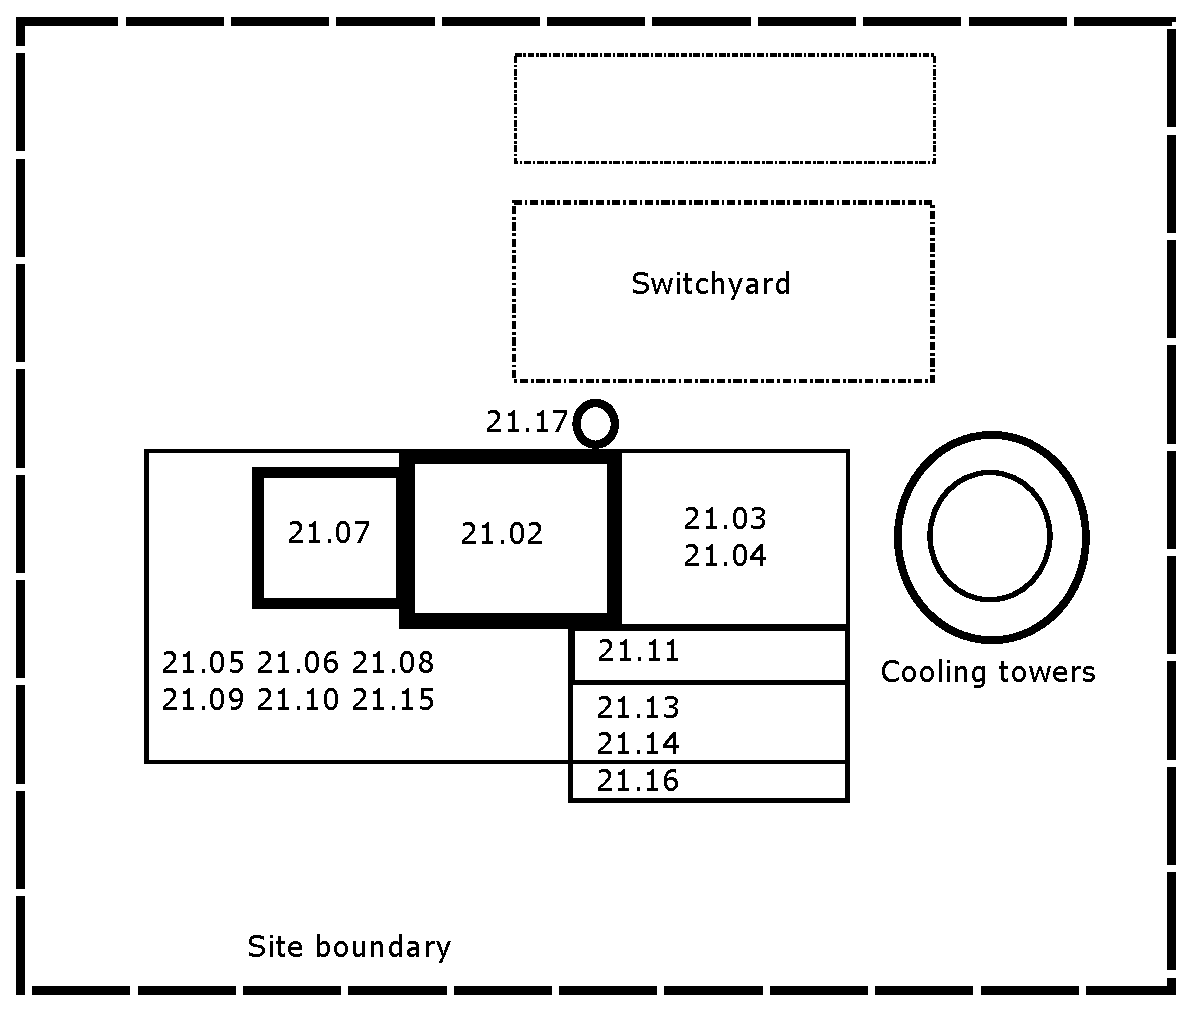
\includegraphics[scale=0.6]{StandardFigures/siteplan2023.eps} 
\caption{Site plan with labels according to the cost accounts described in the text.  Cooling towers and Switchyards are costed elsewhere.} 
\label{fig:site} 
\end{figure} 



 \textbf{2020 Update} 
\emph{Scope: } 
Site preparation and yard work, reactor building, turbine building, security building and gatehouse, control and administrative buildings, maintenance shop, any other site structures and facilities. 
 \emph{Previous values:} CAD calculations for building volumes and concrete volumes multiplied by materials costs. 
Min \$373/kW, Average \$606/kW, Max \$1,142/kW. 
\emph{Reduction strategies: } 
Minimal reactor building size and wall/ceiling thickness (while fully preserving safety); minimal volumes for concrete and other materials (expensive concrete vs. inexpensive soil or sand, perhaps as inner fill material within metal or concrete walls); avoidance of unnecessary buildings in plant design; reuse of buildings if an existing power plant site; modular construction, as in Wartsila Modular Block. 
\emph{Updated value: } 
Average of previous value reduced by 25 \% with implementation of feasible strategies listed above. \$606/kW $\times$ - 0.25 = \$470/kW, giving a total for CAS21 of 111 M \$. 
%\emph{2023 Updated value: } 
%Buildings now built using a bottoms up approach, totaling 450.0 M \$.    
%\begin{figure}[h!] 
%\centering 
%\includegraphics[width =1\linewidth]{/home/ahigginbottom/Desktop/CODE050202023/CATF_DT/MIf_site(1).pdf} 
%\caption{Site, buildings built from the ground up and costed individually.} 
%\label{fig:site} 
%\end{figure} 

\begin{table}[h!] 
    \begin{tiny}
    \centering
    \begin{tabular}{l l  c c c c c c c c c }
Cost Category	&	Building	&	Wall materials	&	 \$/kW gross	&	L	&	W	&	H	&	Vol	&	Esc year	&	Esc	&\$/kW gross	\\
21.01.00	&	Site improve. \& facs	&		&	20.7	&		&		&		&		&	2019	&	1.19	&	24.6	\\
21.02.00	&	Heat Island Building	&	Concrete \& Steel	&	131.6	&	48.3	&	48.3	&	60	&	140000	&	2009	&	1.42	&	186.8	\\
21.03.00	&	Turbine building	&	Steel 	&	45.3	&	48.3	&	48.3	&	30	&	70000	&	2019	&	1.19	&	54.0	\\
21.04.00	&	Heat rejection 	&	Concrete \& Steel	&	31.7	&	48.3	&	48.3	&	15	&	35000	&	2019	&	1.19	&	37.8	\\
21.05.00	&	Power supplies	&	Concrete \& Steel	&	9.1	&	9.7	&	9.7	&	6.0	&	560	&	2019	&	1.19	&	10.8	\\
21.06.00	&	Plant aux.	&	Concrete \& Steel	&	4.5	&	4.8	&	4.8	&	3.0	&	70	&	2019	&	1.19	&	5.4	\\
21.07.00	&	Hot cell	&	Concrete \& Steel	&	65.8	&	24.2	&	24.2	&	60	&	35000	&	2013	&	1.42	&	93.4	\\
21.08.00	&	Heat Island Services	&	Steel frame	&	13.2	&	4.8	&	4.8	&	10	&	233	&	2013	&	1.42	&	18.7	\\
21.09.00	&	Service water	&	Steel frame	&	0.2	&	1.3	&	4.0	&	4.0	&	21	&	2019	&	1.19	&	0.3	\\
21.10.00	&	Fuel storage	&	Steel frame	&	0.9	&	5.0	&	15.0	&	2.5	&	188	&	2019	&	1.19	&	1.1	\\
21.11.00	&	Control room	&	Steel frame	&	0.7	&	4.0	&	12.0	&	2	&	96	&	2019	&	1.19	&	0.9	\\
21.12.00	&	Onsite AC power	&	Steel frame	&	0.7	&	3.6	&	10.8	&	1.8	&	70	&	2019	&	1.19	&	0.8	\\
21.13.00	&	Administration	&	Steel frame	&	3.7	&	20.0	&	60.0	&	10	&	12000	&	2019	&	1.19	&	4.4	\\
21.14.00	&	Site services	&	Steel frame	&	1.3	&	7.3	&	22.0	&	3.7	&	593	&	2019	&	1.19	&	1.6	\\
21.15.00	&	Cryogenics	&	Steel frame	&	2.0	&	11.0	&	33.0	&	5.5	&	2003	&	2019	&	1.19	&	2.4	\\
21.16.00	&	Security	&	Steel frame	&	0.7	&	4.0	&	12.0	&	2	&	96	&	2019	&	1.19	&	0.9	\\
21.17.00	&	Ventilation stack	&	Steel \& concrete 	&	22.7	&		&		&	120	&		&	2019	&	1.19	&	27.0	\\
21.98.00	&	Spare parts allowance	&		&		&		&		&		&		&		&		&	0.0	\\
21.99.00	&	Contingency allowance	&		&	0.0	&		&		&		&		&		&		&	0.0	\\
21.00.00	&	Structures and site facs	&		&	354.9	&		&		&		&		&		&		&	470.7	\\
    \end{tabular}															
    \end{tiny} 																	
    \caption{Cost categories for buildings, and their cost estimation}	
    \label{tab:buildings}
\end{table} 











\subsection*{Cost Category 21.1 Site Preparation/Yard Work}
Includes clearing, grubbing, scraping, geo-technical work, site cut, fill and compact, drainage, fences, landscaping, etc.  Cost is \$ 6 M using NETL Reference case B12A, account 13, bare erected costs for 13.1 site preparation and 13.2 site improvements, for a 686MW gross power plant in 2019 \$, applying escalation per table \ref{tab:buildings}.

\subsection*{Cost Category 21.2 Heat Island Building}
Includes installation, labor, and materials for concrete and metalwork for the building surrounding and supporting the heat island, including the containment structure. Also includes the biological shielding, structural excavation and backfill, foundations, walls, slabs, siding, roof, architectural finishes, elevators, lighting, HVAC (general building service), fire protection, plumbing, and drainage. Cost is \$ 44 M using Waganer cost reference for ARIES-ST.


\subsection*{Cost Category 21.3 Turbine Generator Building}
Includes installation, labor, and materials for concrete and structural metalwork for the building surrounding and supporting the turbine generator(s). (For concepts that do not produce electricity, this account can be replaced with appropriate energy product buildings.) Also includes structural excavation and backfill, foundations, walls, slabs, siding, roof, architectural finishes, elevators, lighting, HVAC, fire protection, plumbing, and drainage.  This building contains the turbines and heat exchangers. Cost is \$ 13 M using NETL Reference case B12A, account 14.3, turbine building bare erected costs for a 686MW gross power plant in 2019 \$, apply escalation per table \ref{tab:buildings}.

\paragraph{}
The rest of the 21 series accounts are for other support buildings on the site. Modular concepts might have a separate building to house centralized functions for all modules, such as an external control room. Here, the building costs are for the complete civil structure, including structural excavation and backfill, foundations, finishes, and building services such as elevators, lighting, HVAC, fire protection, or domestic water and drainage, but do not include the specialized equipment within.

\begin{itemize}
\item Cost Category 21.04 - Heat Rejection Building. This account covers the costs associated with the systems needed for rejecting heat from the power plant, scaled to the rejected thermal power. Cost is \$ 9 M using NETL Reference case B12A, account 14.2, boiler building bare erected costs for a 686MW gross power plant in 2019 \$, apply escalation per table \ref{tab:buildings}. 
\item Cost Category 21.05 - Electrical Equipment \& Power Systems Building. It includes the costs for all electrical equipment and power systems, scaling with the net electrical power output of the plant. Cost is \$ 3 M, using a smaller version of the turbine building - multiple floors, concrete, per table \ref{tab:buildings}.
\item Cost Category 21.06 - Plant Auxiliary Systems Building. This account addresses the costs of auxiliary systems in the plant, such as compressed air, inert gas storage, and distribution systems, scaling with the gross electrical power. Cost is \$ 1 M as smaller version of the turbine building - multiple floors, concrete, per table \ref{tab:buildings}. 
\item Cost Category 21.07 - Hot Cell Building. The cost for the Hot Cell Building, designed for handling large and hazardous components, is scaled in relation to the Reactor Building.  Cost is \$ 22 M as a smaller version of the Heat Island Building by 50\%, per table \ref{tab:buildings}.  
\item Cost Category 21.08 - Heat Island Service Building. This includes the costs for a service building specific to the reactor, similar in cost to structures in projects. Cost is \$ 4 M as smaller version of the Heat Island Building by 10\%, per table \ref{tab:buildings}.  
\item Cost Category 21.09 - Service Water Building. The Service Water Building, essential for the plant’s water supply needs, has its costs modeled after similar structures in other power plant projects. Cost is \$ 0 M following NETL Reference case B12A, account 14.5, circulation water pumphouse and 14.6 water treatment building bare erected costs for a 686MW gross power plant in 2019 \$, applying escalation per table \ref{tab:buildings}.
\item Cost Category 21.10 - Fuel Handling and Storage Building. This account covers the costs for buildings related to handling and storing fuel, scaled according to tritium usage or fusion power. Cost is \$ 0 M, scaled relative to the administration building per table \ref{tab:buildings}. 
\item Cost Category 21.11 - Control Room Building. It encompasses the expenses for the control room building, essential for plant operations, with costs similar to those in previous plant designs.  Cost is \$ 0 M scaled relative to the administration building per table \ref{tab:buildings}. 
\item Cost Category 21.12 - On-Site AC Power Building. This account includes the costs for buildings housing on-site alternating current (AC) power systems, comparable to similar structures in other projects.  Cost is \$ 0 M scaled relative to the administration building per table \ref{tab:buildings}. 
\item Cost Category 21.13 - Administrative Building. It covers the costs associated with the construction of the plant’s administrative building, with cost estimates based on previous similar projects. Cost is \$ 1 M as NETL Reference case B12A, account 14.4, administration building building bare erected costs for a 686MW gross power plant in 2019 \$, apply escalation per table \ref{tab:buildings}. 
\item Cost Category 21.14 - Site Service Building. This account entails the costs for a building providing various site services, with costs aligned with those in comparable plant designs. Cost is \$ 0 M as NETL Reference case B12A, account 14.7, machine shop building bare erected costs for a 686MW gross power plant in 2019 \$, apply escalation per table \ref{tab:buildings}. 
\item Cost Category 21.15 - Cryogenic and Inert Gas Storage Building. It includes the costs for buildings that store cryogenic and inert gases, essential for plant operations.  Cost is \$ 1 M Like site services, per table \ref{tab:buildings}. 
\item Cost Category 21.16 - Security Building. The Security Building account covers the costs for structures dedicated to the plant’s security and surveillance. Cost is \$ 0 M like administration, see table \ref{tab:buildings}. 
\item Cost Category 21.17 - Ventilation Stack. This account addresses the costs of the ventilation stack, a crucial component for plant ventilation and safety. Cost is \$ 6 M as NETL Reference case B12A, account 7, ventilation stack bare erected costs for a 686MW gross power plant in 2019\$, apply escalation per table \ref{tab:buildings}.
\end{itemize}










%%12/7/2023 need an iteration or two

\subsection{Cost Category 22: Heat Island Plant Equipment}

This category is most dependent on the heat island technology being considered, because the sub-account descriptions and costs depend heavily on the coolant used and whether the subsystems are factory-produced or constructed onsite. \\

For the mechanical components, costs are determined by making a CAD drawing of the components  and determining the volume of the component.  The following equation is then used to determine 
component costs from the volumes: $\Sigma_{i} C_{i} = V_{i}  \rho_{i}c_{i}$, where $\rho$ is  the mass density in kg/m$^{3}$ and $c_{i}$ is the cost per unit mass in \$/kg (see Table \ref{tab:materials})  with manufacturing factor applied.

\begin{table}[h!]
\centering
\resizebox{0.7\linewidth}{!}{%
\begin{tabular}{lccccc}
\hline
Material & \(\rho\) (kg/$m^{3}$) & \(c_{\text{raw}}\) (\$/kg or \$/kAm) & Manufacturing Factor & \(\sigma\) (MPa)& \(c\) (\$/kg or \$/kAm)\\
\hline
FS & 7470 & 10 & 3 & 450 & \\
Pb & 9400 & 2.4 & 1.5 & & \\
Li$_4$SiO$_4$ & 2390 & 1 & 2 & & \\
Flibe & 1900 & & & & 40 \\
W & 19300 & 100 & 3 & & \\
Li & 534 & 70 & 1.5 & & \\
BFS & 7800 & 30 & 2 & & \\
PbLi & 8594.0 & & & & 12.82 \\
SiC & 3200 & 14.49 & 3 & & \\
Inconel & 8440 & 46 & 3 & & \\
Cu & 7300 & 10.2 & 3 & & \\
Polyimide & 1430 & 100 & 3 & & \\
YBCO & 6200 & & & & 55 \\
Concrete & 2300 & 0.52 & 2 & & \\
SS316 & 7860 & 2 & 2 & 900 & \\
Nb$_3$Sn & & & & & 5 \\
Incoloy & 8170 & 4 & 2 & & \\
GdBCO & & & & & \\
He & & & & & \\
NbTi & & & & & \\
\hline
\end{tabular}}
\caption{Properties of materials used in fusion reactors.}
\label{tab:materials}
\end{table}


\subsubsection{Cost Category 22.01: Heat Island Components}

The fusion system comprises various critical components, each playing a unique role in ensuring the effective and safe operation of the fusion process. These components are:

\begin{itemize}
    \item Cost Category 22.01.01 First Wall and Blanket. The first wall and blanket are crucial for protecting the reactor's interior from intense fusion reactions and for capturing and converting fusion energy into heat.
    
    \item Cost Category 22.01.02 Shield. The shield serves to protect surrounding structures and personnel from radiation produced during fusion, playing a key role in ensuring safety and regulatory compliance.
    
    \item Cost Category 22.01.03 Magnets. In magnetic fusion systems, magnetic field coils are used to confine and control the fusion reaction.
    
    \item Cost Category 22.01.04 Supplemental Heating. This includes additional heating systems that assist in raising the plasma temperature to the required level for fusion to occur.
    
    \item Cost Category 22.01.05 Primary Structure and Support. The primary structure and support systems provide the necessary mechanical integrity and stability to the fusion reactor.
    
    \item Cost Category 22.01.06 Vacuum System. The vacuum system maintains the necessary vacuum conditions within the reactor chamber, which is crucial for the containment and control of the plasma.
    
    \item Cost Category 22.01.07 Power Supplies. These are essential for providing the electrical power needed for various reactor systems, including heating, cooling, and plasma confinement.
    
    \item Cost Category 22.01.08 Exhaust/divertor. In magnetic fusion systems, the exhaust gases are channeled to a surface called a divertor.

    \item Cost Category 22.01.09 Direct energy convertor. In some cases,energy can be directly converted from the exhaust plasma to electricity with higher conversion efficiency.
    
    \item Cost Category 22.01.11 Assembly and Installation. This encompasses the human resources involved in the assembly and installation of the fusion heat island components.

    \item Cost Category 22.01.19 Scheduled replacement costs.  Capitalized costs of components that will not serve the lifetime of the plant and be replaced on a schedule - usually the first wall and blanket, but can be other components in the heat island.
 \end{itemize}


Each of these major costs are examined in detail in the following sections.
\subsubsection*{Cost Category 22.01.01 First Wall and Blanket} 

The first wall in a fusion heat island serves as a direct interface with the plasma, tasked with withstanding extreme heat and particle flux while also resisting radiation damage and managing tritium retention. The blanket surrounding the first wall plays a dual role in absorbing neutrons to generate heat and breed tritium for fuel, in addition to providing crucial radiation shielding for the reactor's structural integrity and safety.  This Cost Category therefore consists of the following subcategories:

%https://docs.google.com/spreadsheets/d/1SlP_hoDTWUznvav6WUs5kozBXcQWKO2okvEGQukS6Mw/edit#gid=476735038

\begin{itemize}
    \item Cost Category 21.01.01 First wall: the interior surface of the fusion chamber that directly faces the plasma and is subject to extreme conditions. It endures intense heat and particle flux, necessitating the use of materials like refractory metals or specialized alloys that can withstand high temperatures and minimize erosion from particle bombardment. The first wall must also resist radiation damage, particularly in deuterium-tritium fusion reactors, where neutron radiation can cause materials to become brittle and lose structural integrity. An important consideration is the management of tritium retention and release, as wall materials should prevent buildup while allowing efficient extraction and reuse. Additionally, the first wall faces significant thermal stress due to the cyclic nature of fusion reactions, requiring a design that can accommodate stresses without cracking or deforming. Finally, it must be compatible with the cooling system, which could involve water, liquid metal, or other coolants, to ensure effective heat removal. The design and performance of the first wall are critical for the reactor's efficiency, safety, and longevity, which presents a complex engineering challenge that balances heat resistance, structural integrity, and minimal plasma interaction.
    \item Cost Category 21.01.02 Blanket: a crucial component that surrounds the plasma, serving multiple roles. It absorbs neutrons generated during fusion reactions, converting their kinetic energy into heat, and acts as a breeding ground for tritium, an essential fuel in deuterium-tritium fusion reactions, through interactions with materials like lithium. The blanket also provides critical radiation shielding, protecting reactor components and personnel from intense neutron radiation. Additionally, it plays a role in thermal management, as the heat generated within the blanket is often harnessed to produce steam for driving turbines and generating electricity. This makes the design and material choice for the blanket vital for reactor efficiency and safety, which requires advanced materials and engineering to withstand extreme temperatures and radiation levels.
\end{itemize}

The blanket under consideration has a firstW first wall with a primary coolant consisting of primaryC and secondaryC as the secondary coolant, with neutronM as the neutron multiplier, and a structure primarily consisting of structure1. The radial build dimensions are shown in Table \ref{tab:volumes}, which allow us to determine the volumes of components for costing.  The radial build is shown in \ref{fig:radial}.  \\


\begin{table}[h!]
    \centering
    \begin{tabular}{l c  c c c}
    \hline
        &	Thickness	&	Inner Radius	&	Outer radius	&	Volume		\\
        \hline
Plasma	&	1.1	&	2.2	&	2.2	&	VOL1	m$^{3}$	\\
Vacuum	&	0.1	&	1.3	&	1.3	&	VOL2	m$^{3}$	\\
First Wall	&	0.2	&	1.5	&	1.5	&	VOL3	m$^{3}$	\\
Blanket	&	0.8	&	2.3	&	2.3	&	VOL4	m$^{3}$	\\
Reflector	&	0.2	&	2.5	&	2.5	&	VOL6	m$^{3}$	\\
HT Shield	&	0.2	&	2.7	&	2.7	&	VOL9	m$^{3}$	\\
Structure	&	0.2	&	2.9	&	2.9	&	VOL5	m$^{3}$	\\
Gap	&	0.5	&	3.4	&	3.4	&	VOL7	m$^{3}$	\\
Vessel	&	0.2	&	3.6	&	3.6	&	VOL8	m$^{3}$	\\
LT Shield	&	0.2	&	2.7	&	2.7	&	VOL9	m$^{3}$	\\
Coils	&	1.10	&	4.5	&	3.9	&	VOL10	m$^{3}$	\\
Structure	&	1.11	&	3.9	&	3.9	&	VOL11	m$^{3}$	\\
Gap	&	1.12	&	RAD12I	&	RAD12O	&	VOL12	m$^{3}$	\\
Bioshield	&	1.13	&	RAD13I	&	RAD13O	&	VOL13	m$^{3}$	\\

        \hline
    \end{tabular}
    \caption{Volumes of components in the radial build.}
    \label{tab:volumes}
\end{table}

\begin{figure}
    \centering
    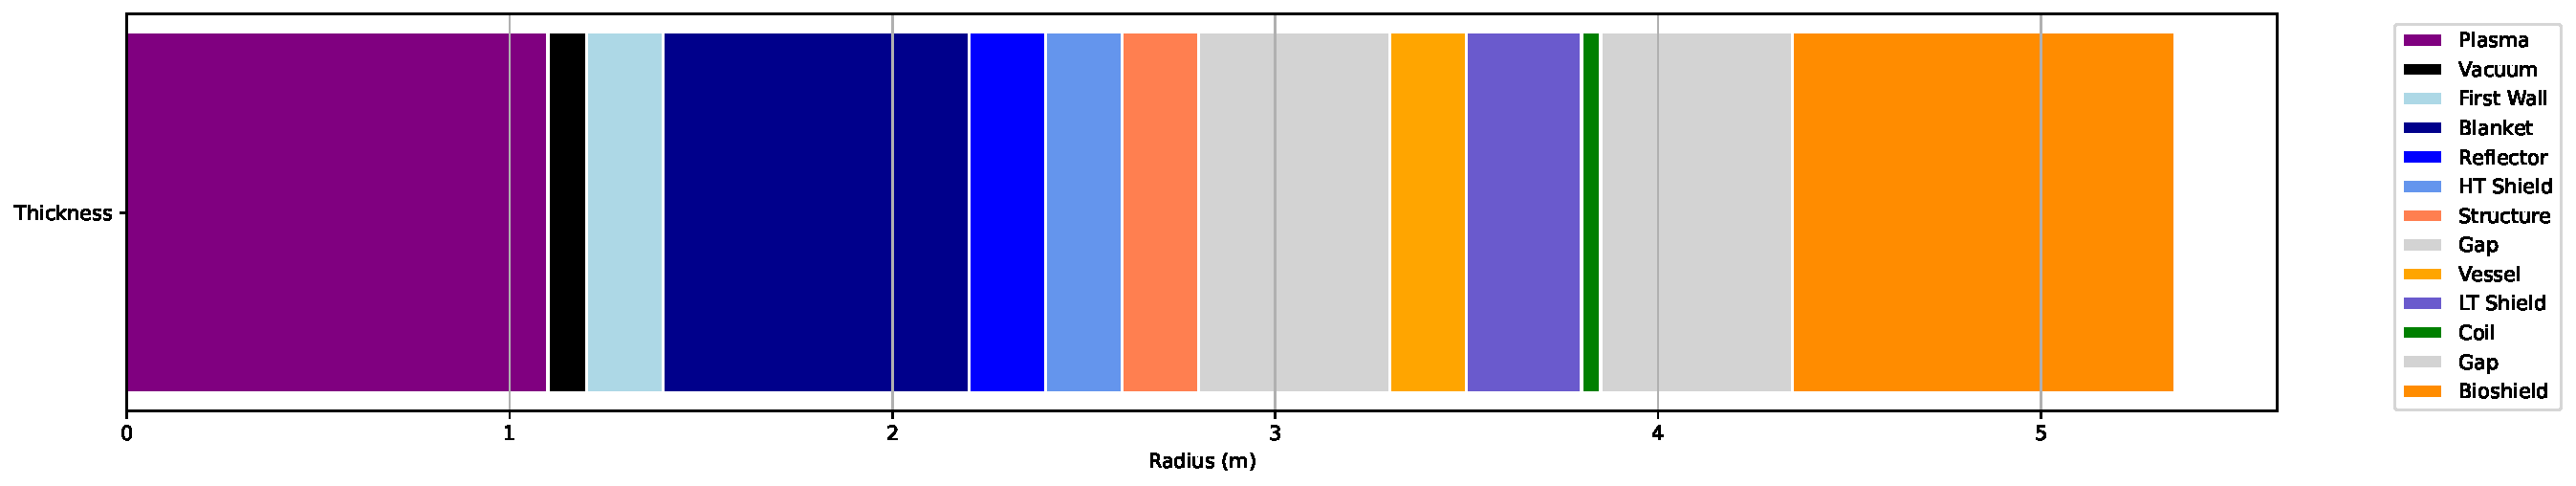
\includegraphics[width=0.9\linewidth]{Figures/radial_build.pdf}
    \caption{Radial build according to Table \ref{tab:volumes}.}
    \label{fig:radial}
\end{figure}



The costs of the first wall and blanket are determined by the volume of the material and multiplied by a manufacturing factor per Table \ref{tab:materials}.   Cost of the first wall is \$ C22010101 M.  Cost of the blanket is \$ C22010102 M.


\subsubsection*{Cost Category 22.01.02: Shield} 

The shield comes in 4 major components - the high temperature shield, the low temperature shield, the bioshield and the penetration shield. Each shield serves a vital role in ensuring both the safety and functionality of the heat island. Primarily, they act as barriers to protect outer components and personnel from the intense neutron radiation and heat generated by the fusion reactions. The shields effectively absorbs and attenuates this radiation, preventing it from causing damage or activating surrounding materials. Additionally, the shields help to maintain the structural integrity of the heat island components and may also play a role in thermal management, capturing and dissipating residual heat. \\

This Cost Category comprises: 

\begin{itemize}
    \item Cost Category 22.01.02.01 High temperature shield consists of a steel structure that envelopes the plasma and blanket system with holes running along the length of the shield for Lead Lithium (PbLi) coolant to flow through, most often placed inside of the vacuum vessel. The basis is determined by the volume of material shown in Table \ref{tab:volumes}, giving a volume of VOL9  m$^{3}$ multiplied by a manufacturing factor, to obtain a cost of \$ 164 M. %Need to pick a cost unit standard, much of the rest used M USD but can switch
    %Waganar has some discussion of other materials including tungsten, boron carbide or borated ferritic steel
    %Also should mention that high temperature shield serves to increase thermal efficency from waste heat captured from adjacent blanket
    %We should mention the total neutron absorption of blanket and shield etc, literature seems to agree on approx 99%
    \item Cost Category 22.01.02.02 Low temperature shielding, which is placed outside of the vacuum vessel and is not cooled.  This structure is usually steel.  The basis is determined by the volume of material shown in Table \ref{tab:volumes}, giving a volume of VOL9  m$^{3}$ multiplied by a manufacturing factor, to obtain a cost of \$ 1 M.
    \item Cost Category 22.01.02.03 Bioshield, typically made of dense, neutron-absorbing materials like concrete, lead, or borated materials, the shield is a crucial component for the safe and efficient operation of a fusion energy system, enabling it to harness the power of fusion while minimizing the associated risks.  The bioshield is computed also from volumes in Table \ref{tab:volumes}, giving a volume of 76 m$^{3}$ and a cost of \$ 3 M. 
    %Should mention the location - text seems to imply exterior to vacuum vessel but Waganar says it can be eithe rin or out, or serve as the structure
    \item Cost Category 22.01.02.04 Penetration shielding consists of the doglegs that are put in place to allow entry or cabling, conduits or coolant systems into the bioshield.  The cost basis is scaled as a relative fraction of the bioshield cost, and so has a cost of \$ 0 M.
\end{itemize}

The total cost for the subsystem is then \$ 168 M.





\subsubsection*{Cost Category 22.01.03: Coils in a Tokamak}

This cost category includes the costing for the plasma confinement coils, including  material, structural and manufacturing cost. As a primary cost driver for this device, careful consideration of a number of parameters is taken, including the number of coils, the conductor material, winding type, and quench mitigation in the case of superconducting cables.\\

\subsubsection*{Cost Category 22.01.03: Coils}

This cost category includes the costing for the plasma confinement coils, including  material, structural and manufacturing cost. As a primary cost driver for this device, careful consideration of a number of parameters is taken, including the number of coils, the B$\times$R value ( in the case of the solenoid coils here), the conductor material, winding type, and quench mitigation in the case of superconducting cables.\\

Consists of:

\begin{itemize}
    \item 22.1.3.1 Toroidal field coils. The toroidal field coils in a tokamak generate a powerful magnetic field that confines the plasma in a stable, donut-shaped loop.
    \item 22.1.3.2 Solenoid coils. The central solenoid in a tokamak functions as a primary electromagnet, creating a magnetic field that initiates the plasma and drives the plasma current.
    \item 22.1.3.3 Poloidal field coils. These are responsible for shaping and stabilizing the plasma, helping to maintain its shape and control its position.
    \item 22.1.3.4 Shim coils. These serve the purpose of making fine adjustments to the plasma to achieve the desired field uniformity or compensate for disturbances.
    \item 22.1.3.5 Structural support. In a tokamak the structure is needed to brace the magnets against torsional forces.
\end{itemize}
   

The approach taken was to compare various geometries of HTS, LTS and copper coil sets using COMSOL, with the same central field and minimum inner radius requirements. These were down-selected to an HTS geometry with 12.0 solenoid coils, and 1.0 inner mirror coils and 2.0 outer mirror coils.\\

To determine the cost, the coil parameters were determined using a combination of COMSOL, calibration points from the literature including Menard 2016 \cite{Menard2016} for HTS, and EU DEMO for LTS, and analytical electromagnetic modeling. The material cost then then be determined through the mass/length (in the case of REBCO tape) of each material used. \\

To cost the magnet system, two steps are required. The first is to have the specifications of the magnets required, and the second is to calculate the resulting material requirements and costs, with a manufacturing factor applied to this total. In the costing code provided, four basic magnet types are available: HTS (CICC), HTS (pancake), LTS (CICC) and copper. In the standard code, as arguably the new industry standard, only HTS (CICC) includes both both steps of design and costing. For all others, the user will need to provide the following basic specifications to input into the code for a cost to be returned:

\begin{itemize}
    \item Magnet coil counts: this input specifies the number of identical coils of each type.
    \item Magnet type: specifies the magnet type of the four described above.
    \item \textit{r} centre: the average radius of the coil.
    \item \textit{z} centre: the displacement of the centre of the coil in the \textit{z} (vertical) axis.
    \item \textit{dr}: the radial thickness of each coil.
    \item \textit{dz}: the thickness of each coil in the \textit{z} axis.
    \item Insulating material fraction: in the case of the pancake winding geometry, a "partial insulation" is used. Currently, the 'partial insulation' technology being developed by, for example, Tokamak Energy is proprietary and details are not publicly available. As such, for costing purposes, a fraction of fracIns of the total cross-sectional area is assumed to be insulating material, with a density similar to paraffin or epoxy, and a material cost of 20.0 \$/kg. These values are purely indicative of an order-of-magnitude costing reference, and can be updated with more information as costing code inputs.
    \item Manufacturing factor: a scalar multiplying factor which is applied to the total material cost of each coil, based upon the complexity and cost of winding and installing the coil. Default values are provided for each coil type. For HTS, for example, there has yet to be a commercially implemented CICC, so it is assumed that the cost of winding is comparable with that of LTS, which is widely available. 
    \item Structural factor: another scalar multiplying factor applied to the total cost of the magnet (including manufacturing factor). This accounts for the direct structure required to support each magnet. Default values are provided here too, varying approximatley from 25-100\% of the base cost of the magnet.
\end{itemize}

For the purposes of clarity, and as a methodology guide for other coil types, the design approach for step 1 of the HTS (CICC) coils is as follows. The coil geometries and specifications as described in Menard 2016 \cite{Menard2016} as used as a calibration point. These specifications are then input into a Biot-Savart code that calculates the field at given coordinates. The coil is considered to comprise of N turns of current-carrying circular loops, with varying radii and \textit{r} and \textit{z} displacements. The total contributions of each concentric turn are then summed to determine the central field at \textit{r = 0}.\\

Using these data, a SciPy interpolation function is used to determine the coil specifications required to achieve a given central field, constrained by the required average radius.\\

It should be noted that the default cable geometry as seen in \href{fig:yuhu_cs} is by no means optimised, and it is recommended that for minimal capital costs, a minimal length of REBCO and a maximum available current is used.


\begin{figure}[h]
    \centering
    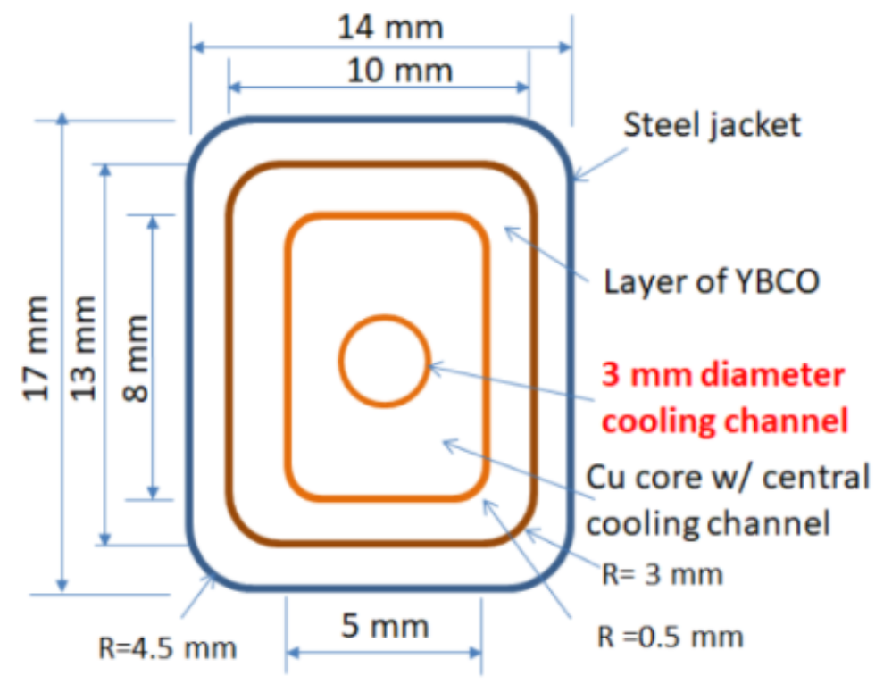
\includegraphics[width =0.5\linewidth]{StandardFigures/yuhu_cs.pdf}
    \caption{HTS cable geometry.}
    \label{fig:yuhu_cs}
\end{figure}

Another recommended approach is to employ a multi-physics FEM tool such as COMSOL to design the magnet with the required properties to obtain the inputs required for the costing code.

It should be noted that a series of optimizations can be made to the design to reduce cost. The first of these is conductor grading. By reducing the number of strands of superconductor where the fields lower, up to 50\% of the superconducting material can be saved \cite{uglietti2018progressing}.\\

The total cost of the coils is 1000.0 M USD.


\subsubsection*{22.1.3.1 Toroidal Coils}

This design consists of notfcoils toroidal field coils, which can be individually removed for maintenance. The total cost is \$110.0 M.\\

Both LTS and HTS cables can be considered here. For each, a wide variety of designs are available, including no-insulation, partial insulation, and an array of CICC geometries. For this concept, a simple CICC geometry is considered \cite{Menard2016}, comprising a layer of superconducting REBCO conductor, copper for quench mitigation and cooling, a central coolant channel, and a steel jacket to help resist the considerable forces experienced during operation. See \ref{fig:yuhu_cs} for the specific geometry.\\

To cost the system, the magnet specifications are calibrated against \cite{Menard2016}, and extrapolated to the requirements of this concept. The total length of the conductor is then calculated and, assuming a cost of 12 \$/kAm, the total cost can be found. For the steel and copper, the volume is also found and multiplied by the cost per kilogram. This gives a total material cost for the coil, which is then multiplied by a manufacturing factor. The manufacturing factor comprises the cost of manufacturing the cables, then winding and installing the coils. 

\subsubsection*{22.1.3.2 Central solenoid}

For the central solenoid, either LTS or HTS cables are viable. In this case, the HTS geometry as seen in \ref{fig:yuhu_cs} is used. The total cost is \$12.0 M.

\subsubsection*{22.1.3.3 Poloidal Coils}

This subsystem includes 16.0, corresponding to 8.0 pairs of identical pairs, displaced in positive and negative z coordinates. Owing to the generally large radius, HTS and LTS coils must be considered here. In this case, HTS coils are used, owing to their significantly increased current density, reducing the required number of turns and length of superconductor. This allows for a reduced form factor for the entire system, resulting in a multiplicative cost saving. The cable geometry used here is described in \ref{fig:yuhu_cs}, although other HTS CICC geometries may be more optimised.
Since the lower PF coils are effectively trapped by the TF coils and the power core above them, additional spare PF coils are to be provided below the power core. Even though the PF coils are designed to be life of plant and replaceable, the downtime to replace these particular lower PF coils are so onerous, it is more cost effective to have spares installed during the initial build sequence.  \\

The total cost of the PF coils is \$700.0 M. 

\subsubsection*{22.1.3.4 Shim Coils}

These coils serve to apply fine adjustments to the field profile to maintain field uniformity, and control any plasma disturbances. The placement, size, and magnitude of these coils is dependent upon the uniformity requirements of the plasma, and requires sophisticated FEM analysis to accurately quantify. As such, for the scope of this costing report, a simple factor of 5\% of the total primary magnet costs is taken. The resulting cost is \$41.0 M.

\begin{table}[h]
\centering
\resizebox{\linewidth}{!}{%
\begin{tabular}{lcccccccccc}
\hline
\textbf{Parameter} & \textbf{TF} & \textbf{CS} & \textbf{PF1} & \textbf{PF2} & \textbf{PF3} & \textbf{PF4} & \textbf{PF5} & \textbf{PF6} & \textbf{PF7} & \textbf{PF8} \\
\hline
Magnet Type & HTS CICC & HTS CICC & HTS CICC & HTS CICC & HTS CICC & HTS CICC & HTS CICC & HTS CICC & HTS CICC & HTS CICC \\
Radius (m) & 3.8 & 0.18 & 0.67 & 0.9 & 1.28 & 2.72 & 5.3 & 9.34 & 9.34 & 3.80 \\
dr (m) & 0.25 & 0.2 & 0.3 & 0.3 & 0.5 & 0.75 & 1.8 & 1.0 & 1.0 & 1.0 \\
dz (m) & 0.35 & 6.3 & 0.6 & 0.6 & 0.6 & 0.37 & 0.37 & 1.0 & 1.0 & 1.0 \\
Current supply (MA) & 3.4 & 49.0 & 6.9 & 6.9 & 12.0 & 11.0 & 26.0 & 39.0 & 39.0 & 39.0 \\
Conductor current density (A/mm$^2$) & 150.0 & 150.0 & 150.0 & 150.0 & 150.0 & 150.0 & 150.0 & 150.0 & 150.0 & 150.0 \\
Cable width (m) & 0.014 & 0.014 & 0.014 & 0.014 & 0.014 & 0.014 & 0.014 & 0.014 & 0.014 & 0.014 \\
Cable height (m) & 0.017 & 0.017 & 0.017 & 0.017 & 0.017 & 0.017 & 0.017 & 0.017 & 0.017 & 0.017 \\
Total volume (m$^3$) & 2.1 & 1.4 & 2.1 & 1.4 & 0.76 & 1.0 & 2.4 & 4.7 & 22.0 & 59.0 \\
Cross-sectional area (m$^2$) & 0.087 & 1.3 & 0.18 & 0.18 & 0.3 & 0.28 & 0.67 & 1.0 & 1.0 & 1.0 \\
Turn-turn Insulation Fraction & 0 & 0 & 0 & 0 & 0 & 0 & 0 & 0 & 0 & 0 \\
\hline
Cable turns & 370.0 & 5300.0 & 760.0 & 760.0 & 1300.0 & 1200.0 & 2800.0 & 4200.0 & 4200.0 & 4200.0 \\
Total turns of conductor & 43000.0 & 620000.0 & 89000.0 & 89000.0 & 150000.0 & 140000.0 & 330000.0 & 490000.0 & 490000.0 & 490000.0 \\
Length of conductor (km) & 1000.0 & 700.0 & 370.0 & 500.0 & 1200.0 & 2300.0 & 11000.0 & 29000.0 & 29000.0 & 29000.0 \\
Current per conductor (A) & 78.0 & 78.0 & 78.0 & 78.0 & 78.0 & 78.0 & 78.0 & 78.0 & 78.0 & 78.0 \\
\hline
Cost of REBCO tape(\$/kAm) & 10.0 & 10.0 & 10.0 & 10.0 & 10.0 & 10.0 & 10.0 & 10.0 & 10.0 & 10.0 \\
Cost of SC (M USD) & 0.81 & 0.55 & 0.29 & 0.39 & 0.93 & 1.8 & 8.5 & 23.0 & 23.0 & 23.0 \\
Cost of copper (M USD) & 0.052 & 0.036 & 0.019 & 0.025 & 0.06 & 0.12 & 0.55 & 1.5 & 1.5 & 1.5 \\
Cost of SS (M USD) & 0.021 & 0.014 & 0.0077 & 0.01 & 0.024 & 0.048 & 0.23 & 0.6 & 0.6 & 0.6 \\
Cost of other turn-turn insulation (M USD) & - & - & - & - & - & - & - & - & - & - \\
Total material cost (M USD) & 0.88 & 0.6 & 0.32 & 0.43 & 1.0 & 2.0 & 9.3 & 25.0 & 25.0 & 25.0 \\
Manufacturing factor & 5.0 & 10.0 & 2.0 & 2.0 & 2.0 & 2.0 & 2.0 & 2.0 & 2.0 & 2.0 \\
Structural cost (M USD) & 4.4 & 6.0 & 0.64 & 0.86 & 2.0 & 4.0 & 19.0 & 49.0 & 49.0 & 49.0 \\
Quantity & 12.0 & 1.0 & 2.0 & 2.0 & 2.0 & 2.0 & 2.0 & 2.0 & 2.0 & 2.0 \\
Magnet cost (single)(M USD) & 4.4 & 6.0 & 0.64 & 0.86 & 2.0 & 4.0 & 19.0 & 49.0 & 49.0 & 49.0 \\
Magnet + structure cost (single) (M USD) & 8.8 & 12.0 & 1.3 & 1.7 & 4.1 & 8.0 & 37.0 & 99.0 & 99.0 & 99.0 \\
\hline
Total cost (M USD) & 110.0 & 12.0 & 2.5 & 3.4 & 8.1 & 16.0 & 75.0 & 200.0 & 200.0 & 200.0 \\
\hline
\end{tabular}}
\caption{Design parameters for an individual coil of each of the main coils in this concept.}
\label{your-table-label}
\end{table}


\subsubsection*{22.1.3.5 Structural cost for coils}

The structural cost for the coils is difficult to cost from first principles without detailed structural analysis with FEM. Here, the approach is a series of analytical estimations of the dominant stresses. These include:

\begin{itemize}
    \item Hoop stress within the coil generated by the cumulative effect of the induced force between concentric radial turns.
    \item Axial force generated between cable turns within the coils. 
    \item Axial force between adjacent coils.
\end{itemize}


In the case of Tokamaks, significant torsional forces are induced, demanding considerable bracing structure. By considering these primary contributions, an estimate of the structural material required (such as the hoop restraint requirements) can be calculated. From this preliminary estimate, a structural cost of 100\% of the coil cost is used as a conservative factor, based on previous Tokamak structural costs. The structural cost is thus 180.0 M USD.



\subsubsection*{Cost Category 22.01.04: Supplementary Heating Systems.}

Supplementary heating systems in fusion, such as neutral beam injection and radio frequency (RF) heating, are critical for achieving the necessary plasma conditions for fusion. Neutral beam injection involves injecting high-energy neutral atoms into the plasma, on the other hand, RF heating uses electromagnetic waves to transfer energy to the plasma. These systems are essential for heating the plasma to the extremely high temperatures required for fusion reactions to occur efficiently.\\

Supplementary heating systems contains costs associated with heating and current drive systems, including 

\begin{itemize}
    \item 22.01.04.01 Neutral Beam Heating.   Neutral Beam Injection (NBI): This method involves injecting high-energy neutral atoms (typically hydrogen or deuterium) into the plasma. These neutral atoms penetrate the magnetic fields and, upon ionization, transfer their energy to the plasma particles, thereby heating the plasma.
    \item 22.01.04.02 RF Heating.  Radio Frequency (RF) Heating: Uses electromagnetic waves to transfer energy directly to the plasma particles. Common methods include Ion Cyclotron Resonance Heating (ICRH), where ions absorb energy from the RF waves, and Electron Cyclotron Resonance Heating (ECRH), which targets electrons.
    \item 22.01.04.03 Laser heating.  Can include laser heating of Maglif targets, or precursor lasers for shaping of the target.
    \item 22.01.04.04 Other heating.  Can include schemes like novel electrostatic (biasing electrodes, pulsed, or oscillating electric fields) or time-varying magnetic (e.g. transit-time magnetic pumping).
\end{itemize}


The concept presented here will employ both NBI and ICRF supplementary heating systems. By comparing with prior studies (see table \ref{tab:supp_heat}), a top-down estimation can be found for each. For a NBIPOWER MW NBI system, the cost is 353 M USD, and for a 0 MW ICRF, the cost is 0 M USD, totalling 353 MUSD for the system.

\begin{table}[htbp]
    \centering
   
    \begin{tabular}{lcccrr}
        \hline
        System & Type & Power (MW) & \$/W (2009) & \$/W (2023) \\
        \hline
        ARIES-AT & ICRF/LH & 37.4 & 1.67 & 2.39 \\
        ARIES-I & ICRF/LH & 96.7 & 1.87 & 2.67 \\
        ARIES-I' & ICRF/LH & 202 & 1.96 & 2.80 \\
        ARIES-RS & ICRF/LH/HFFW & 80.8 & 3.09 & 4.42 \\
        ARIES-IV & ICRF/LH & 68.0 & 4.35 & 6.22 \\
        ARIES-II & ICRF/LH & 66.1 & 4.47 & 6.39 \\
        ARIES-III' & NBI & 163 & 4.93 & 7.05 \\
        ARIES-III & NBI & 172 & 4.95 & 7.08 \\
        ITER & ICRF & & 5.5 & 7.87 \\
        Average &  & 110 & 3.64 & 5.21 \\
        Average (ICRF) &  & 91.9 & 2.90 & 4.15 \\
        Average (NBI) &  & 167 & 4.94 & 7.06 \\
        \hline
    \end{tabular}
     \caption{Power and Cost Data (Rounded to 3 Significant Figures)}
    \label{tab:supp_heat}
\end{table}


\subsubsection*{Cost Category 22.01.05:  Primary Structure and Support}
\label{sec:22.1.5}
This account defines the cost of the primary structure and support for the power core. This subsystem  transfers the gravity and seismic loads to the building support structures. Elements include reactor pressure vessel supports, brackets, sealings, pipe supports, or others, including shielding materials if they are integral parts of the support structure. \\

A key requirement of the primary support structure is to absorb and mitigate seismic loads. When building nuclear fission reactors, the accounting of seismic events has been a key cost driver. This is because near-surface soils and seismic hazard are different at each site, requiring site-specific analysis, design, engineering, qualification, licensing, and regulatory review, essentially making every design First-of-a-Kind (FOAK). Thus, a standardized approach is required to mitigate this cost for wide-scale, multiregion fusion reactor deployment. \\

The cost of this category has been largely based on a survey of the structural costs of nuclear fission conducted by Lal et al. \cite{lal2022towards}. Costs associated with this system can be broken into the following. 
\begin{itemize}
    \item 22.02.05.01 Engineering costs. This includes . The cost to analyze/design for operational loadings and calculate its seismic capacity, the cost to seismically qualify the first unit, the cost to prepare for, and of, regulatory review.
    \item 22.02.05.02 Fabrication costs. This includes the cost to fabricate the first unit, including materials, tooling, etc., the cost to fabricate the tenth unit identical to the first unit, the cost to increase seismic capacity of the first unit for the specified peak ground acceleration (PGA) required for the region. This includes all costs of analysis, design, seismic qualification, and peak ground acceleration regulatory review, and the cost to fabricate the first unit with seismic capacity associated with the required PGA. 
\end{itemize}

It has been shown \cite{lal2022towards} that the costs for this category are significantly impacted by the seismic load, and decreasing the PGA at the reactor, greatly reduces costs. One means for isolation is to mount the reactor on numerous concave Friction Pendulum (FP) bearings. By employing these FP bearings, a cost saving of 40-50\% can be achieved \cite{lal2022towards}.\\

For the reactor core, the average costs for a FOAK reactor from 11 facilities can be found for each construction step for a 1000MW reactor core.\\

To cost the system in this report, these costs are scaled to the system power, 518 MW, with a learning credit applied due to the EoS gained by standardised manufacturing, and a consideration of the likely maximum PGA for the location the reactor is constructed in. The final costs are \$ 7101 M for engineering and \$ 7102 M for fabrication, totaling \$71 M for the subsystem in the specified region, assuming a PGA of 0 g.

\subsubsection*{Cost Category 22.1.6: Vacuum System}

The vacuum system in a nuclear fusion reactor plays a critical role in creating and maintaining a high-quality vacuum environment essential for plasma containment and fusion reactions. It comprises various components such as vacuum vessels, primary and roughing vacuum pumps, helium liquefier-refrigerators, and vacuum ducts, each contributing to the effective evacuation and thermal management necessary for sustained and controlled fusion processes. Cost Category 22.1.6 Vacuum System consists of:  

\begin{itemize}
\item 22.1.6.1 Vacuum Vessel.  The vacuum vessel is a sealed container designed to maintain a high vacuum environment, essential for minimizing interactions between the plasma and any residual gases, thus enabling controlled fusion reactions.

\item 22.1.6.2 Helium Liquefier-Refrigerators. Helium liquefier-refrigerators are used to cool components of the reactor, such as superconducting magnets, to extremely low temperatures, often necessary for maintaining superconductivity and efficient thermal management.

\item 22.1.6.3 Primary Vacuum Pumps. Primary vacuum pumps are responsible for creating and maintaining the vacuum within the vessel by removing gases and air, which is crucial for the initial establishment of the vacuum environment.

\item 22.1.6.4 Roughing or Backing Pumps. Roughing or backing pumps are used in conjunction with primary vacuum pumps, typically to provide the initial evacuation of the vessel and reduce the pressure to a level where primary pumps can operate effectively.

\item 22.1.6.5 Vacuum Ducts. Vacuum ducts are the conduits that connect various components of the vacuum system, facilitating the efficient transport and removal of gases from the vacuum vessel to the pumps.
\end{itemize}

Each subsystem is considered in detail as follows. \\
%(see \ref{tab:subsystem_cost_plainvars})

22.1.6.1 Vacuum vessel: this account dominates the cost of the vacuum system and includes only the structural elements of the vacuum system, including the main vacuum vessel chamber, port enclosures, the vacuum door assembly, bulk shielding inside the walls of the vacuum vessel and any manifold / padding \cite{waganer2006design}. It serves two primary functions: (1) to maintain the vacuum environment created by the pumping system for the plasma experiments; (2) to provide the structural support for the superconducting magnets and the other internal and external systems. The design for this mirror concept is based on the vessel used for the MFTF-B at LLNL \cite{gerich1986design}. \\

The vacuum vessel serves as a  key structural element in the reactor, from which other systems including coils and cryogenic systems are mounted.  As such, there are several key loading requirements:

\begin{itemize}
    \item Gravity load. The vessel must support the 1 g force acting straight down on the entire vessel and the components it supports. The dominant masses are the vessel itself 71993 tonnes, the total coil mass COILM tonnes, and auxiliary components inside and outside the vessel, 500 tonnes.

    \item External pressure load. The external pressure load is caused by the standard atmospheric pressure acting on the vessel shell when the vessel is under vacuum, plus an additional 10\% of the atmospheric load to account for magnetic  pressure on the shell resulting from the sudden collapse of the magnetic field. 

    \item Thermal cooldown load. The thermal cooldown load is  caused by the magnets cooling to 4 K, while the vessel remains at room temperature. Because the magnets are connected to the vessel by a number of support struts on each  magnet group, the possibility exists for an over-constrained  strut system to generate thermal contraction loads.

    \item Environmental thermal load. The environmental thermal load is caused by the variation in the air temperature surrounding the vessel.

    \item Magnetic loads. There are numerous magnetic loads that need to be accounted for. These are discussed in Section \ref{sec:22.1.5}.
\end{itemize}

When considering the geometry of the coil, a vacuum vessel CAD can be generated to wrap around the set of coils, with the basic design features adapted from MFTF-B \cite{gerich1986design}. The vessel parameters can be seen in table \ref{tab:ves_params}. For the coil geometry specified in Cost Category 22.1.3, a total material volume of 11 m$^3$ is calculated. ASTM A240 Type-304 stainless steel is used because it is nonmagnetic, has good fracture toughness and welding properties, is readily available and inexpensive, and a total mass of 71993 tons is required, costing 0.4 M USD. Considering the manufacturing and assembly process, however, will increase the vessel cost significantly. One notable requirement is to polish the entire inner surface to maintain the required high vacuum, and reduce the risk of electrical faults. An approximate manufacturing factor of 10 is assumed for the entire process. This results in a cost for vacuum vessel of 4 M USD.


\begin{table}[h]
    \centering
    \resizebox{0.4\linewidth}{!}{%
    \begin{tabular}{lc}
    \hline
        Vessel volume (m$^3$) & 1340\\
        Material volume (m$^3$) & 11\\
        Material & ASTM A240 304 SS\\
        Material mass (tons) & 71993\\
        Material cost (M USD) & 0.4\\
        Total cost (M USD) & 4 \\
         \hline
    \end{tabular}}
    \caption{Vacuum vessel parameters.}
    \label{tab:ves_params}
\end{table}


\begin{figure}[h!]
    \centering
    \includegraphics[width=0.75\linewidth]{NovatronFigures/NovatronVV.png}
    \caption{CAD model of the vacuum vessel geometry, with properties as defined in \ref{tab:ves_params}.}
    \label{fig:VVCAD}
\end{figure}





22.1.6.2 Helium Liquefier-Refrigerators: This subsystem is the helium refrigeration and liquefaction process equipment. It is responsible for supplying the cooling necessary to maintain an operation temperature of 20 K at the coils. \\

The costs for this subsystem are 4 M USD for the vacuum vessel, 4 M USD for the cooling systems, 13 M USD for the vacuum pumping systems, and 0 M USD for the roughing pump. The total cost is 21 M USD.\\

To determine the cooling power necessary to maintain 20 K in the coils, an analytical approach is taken, considering the primary heating components at the HTS coils. These are assumed to be the heat conducted through the support structure, and the neutron flux through the blanket (assuming 99\% of the neutron power is captured in the blanket). At 20 K, for one coil, these are estimated to contribute 11.2 and 1.8 kW, respectively. Scaling for a refrigeration efficiency of 15\% of the Carnot efficiency between 300 and 20 K, this results in a room temperature cooling power requirement of 0.01 MW. The operation temperature is selected based on a trade-off of the cooling efficiency (see fig \ref{fig:cool_eff}), and the superconducting properties of the HTS coils.\\

Using STARFIRE as a reference (ITER cryogenic costs seem to be unexpectedly high), the cost for 20 kW of cooling at 4.2 K is 25.2 M USD. Scaling this to the cooling requirements of the system presented here results in a cost of 4 M USD. \\

\begin{figure}[h]
    \centering
    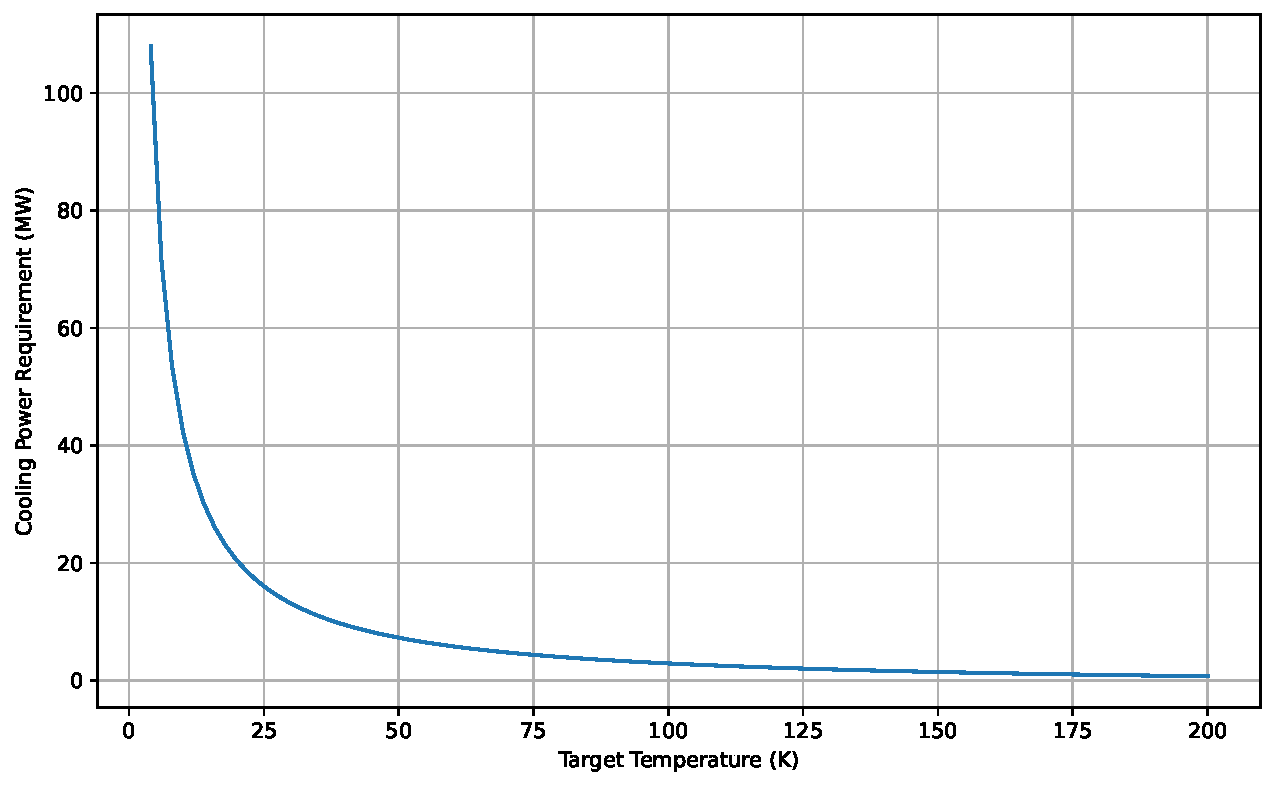
\includegraphics[width=0.75\linewidth]{NovatronFigures/cooling_efficiency.pdf}
    \caption{The cooling power requirement for various magnet operating temperatures.}
    \label{fig:cool_eff}
\end{figure}



22.1.6.3 Primary Vacuum Pumps: consists of d a distributed vacuum subsystem with vacuum pumps located at each sector. For a vacuum of 7694 m$^3$, 1846 vacuum pumps will be required, costing 50 K USD each, corresponding to a total pumping system cost of 13 M USD.\\

22.1.6.4 Roughing Pumps: Consists of a single roughing pump to establish an initial vacuum. Scaled from STARFIRE, this will cost 0 M USD.


\subsubsection*{Cost Category 22.01.07: Power Supplies} 

This category covers an extensive range of power supply systems critical for operation. This includes High-Voltage Power Supplies for plasma heating, Pulsed Power Supply Systems for plasma initiation, and Superconducting Coil Power Supplies for magnetic confinement. Auxiliary Heating Power Supplies support additional plasma heating, while Cooling and Cryogenic Systems maintain optimal temperatures for superconducting components. 


\begin{itemize}
    \item Cost Category 22.07.01 {High-Voltage Power Supplies. Essential for driving heating systems like neutral beam injectors, which heat the plasma to the necessary temperatures for fusion.
    \item Cost Category 22.07.02 Pulsed Power Supply Systems. These provide high-power electrical pulses required for plasma initiation and shaping.
    \item Cost Category 22.07.03 Coil Power Supplies: These are crucial for large superconducting magnets, and copper coils for equilibrium control.
    \item Cost Category 22.07.04 Auxiliary Heating Power Supplies. These are used for additional plasma heating systems like ion cyclotron resonance heating (ICRH) and electron cyclotron resonance heating (ECRH).
    \item Cost Category 22.07.05 Cooling and Cryogenic Systems. To maintain the necessary low temperatures for the superconducting magnets and other components.
    \item Cost Category 22.07.06 Control and Instrumentation Power Supplies. For the myriad of sensors, diagnostics, and control systems involved in monitoring and controlling the fusion reactor.
    \item Cost Category 22.07.07 Power Conversion Systems for Plasma Heating. Such as gyrotrons for ECRH and klystrons or tetrodes for ICRH.
    \item Cost Category 22.07.08 Safety and Interlock Systems. To ensure safe operations, especially during abnormal events or emergencies, these systems can cut power or initiate shutdown sequences.
    \item Cost Category  22.07.09 Diagnostics and Monitoring Systems Power Supply. For real-time monitoring of plasma and reactor conditions, requiring reliable and clean power sources.
\end{itemize}

%need to escalate this cost relative to the 2011 data from ITER:
%https://docs.google.com/spreadsheets/d/1MHiUnJ580Vxzbb7P5V9vQH0PnGHsuDlx/edit?usp=sharing&ouid=106425516412438351916&rtpof=true&sd=true
Cost basis is taken from ITER for a 500MW fusion system, scaling the 269.6kIUA (1kIUA is 2MUSD), giving 539M USD for a 500MW fusion system. The total cost is 79 M USD for a 518 GW fusion system.


%\begin{figure}[h!]
%    \centering
%    \includegraphics[scale=0.4]{LEF_Numx.eps}
%    \caption{Lifetime extension factor vs ratio of applied to rated voltage}
%    \label{fig:1}
%\end{figure}

%\begin{figure}[h!]
%    \centering
%    \includegraphics[scale=0.4]{LOB_Numx.eps}
%    \caption{Lifetime of bank in years, at 1Hz vs ratio of applied to rated voltage}
%    \label{fig:2}
%\end{figure}


%\begin{figure}[h!]
%\centering
%\includegraphics[scale=0.4]{BCF_Numx.eps}
%\caption{Bank cost factor vs ratio of applied to rated voltage}
%\label{fig:3} 
%\end{figure}


\subsubsection*{Cost Category 22.01.08 Divertor}

A divertor in fusion energy systems, particularly used in tokamak reactors, is a critical component designed to handle waste heat and particles from the plasma, crucial for maintaining plasma purity and stability. Positioned at the tokamak's bottom, it acts as an exhaust system, diverting the plasma's impure outer edge into a specialized chamber, thus shielding the reactor's walls from intense heat and particle bombardment. Within this chamber, the plasma cools, and impurities, including helium ash, are extracted. Divertor materials, like tungsten or carbon composites, are selected for their high heat and particle flux tolerance. Advanced divertor designs focus on spreading heat over larger areas to manage the extreme heat flux and enhance the divertor's longevity, making them a vital focus in the ongoing development of sustainable fusion energy technology.\\

Consists of:

\begin{itemize}
    \item Cost Category 22.01.08.01 Divertor Armor. This subsystem deals with the materials used in the divertor's construction, particularly those that can withstand high heat and neutron flux, such as tungsten or carbon-based composites.

\item Cost Category 22.01.08.02 Divertor Magnetic System, coils and components needed to channel and control incident heat flux.

\item  Cost Category 22.01.08.03 Plasma Detachment Subsystem. This involves mechanisms to create a detached plasma state in the divertor region, reducing the heat and particle loads on the divertor surfaces. 


\item Cost Category 22.01.08.04 Pumping and Exhaust Subsystem. This involves the systems required to pump out impurities and heat from the divertor chamber and manage the exhaust of these materials in a controlled manner.

\item Cost Category 22.01.08.05 Diagnostic and Monitoring Subsystem. This includes sensors and diagnostic tools that monitor the performance of the divertor, including temperature, plasma density, and impurity levels. This subsystem is critical for divertor operation control and for informing maintenance and operational adjustments.
\end{itemize}

 The total is thus 133 M USD.

\subsubsection*{Cost Category 22.01.09: Direct Energy Convertor}

A direct energy converter for fusion applications is a groundbreaking advancement in energy technology, notable for its remarkable efficiency of up to 70\% in converting plasma energy to electricity. Key components include the Expander Tank, which reduces the power loading from diverted plasma, and the Expander Coils, essential for directing plasma towards electrodes that convert the energy.  Consists of:

\begin{itemize}
    \item Cost Category 22.01.09.01 Expander Tank. Converts surface power loading to tolerable levels from the diverted plasma to incidents surfaces.
    \item Cost Category 22.01.09.02 Expander Coils.  Provides the magnetic funnel to direct plasma towards surfaces.
    \item Cost Category 22.01.09.03 Neutron Trap.  Provides shielding of components in the direct energy converter from neutron damage.
    \item Cost Category 22.01.09.04 Vacuum System (separate from the chamber vacuum system).  Provides pumping on the direct energy converter.
    \item Cost Category 22.01.09.05 Collector Electrode system.  Allows charged particles to be captured on electrode surfaces for energy to be directly converted.
    \item Cost Category 22.01.09.06 Thermal Management.  Cooling system for electrodes - either passively radiatively or actively with a liquid or gaseos coolant.  Includes heat rejection system.
    \item Cost Category 22.01.09.07 Electrical subsystem.  Provides the coupling to the balance of plant systems, listed in Cost Category 24. Electric Plant Equipment.
\end{itemize}


The collector can accrue damage from sputtering caused by the ion fluence. For tungsten ribbons, this erosion rate is estimated to be 0.02 mm/year, resulting in a low likelihood of having to replace grid elements.\\

Using additively manufactured ribbons with a simple water coolant channel, a heat flux of 2 MW/m$^2$ is acceptable, reducing the overall volume and thus the cost of the subsystem by a factor of 60\% compared with a 1 MW/m$^2$ flux radiatively-cooled system.\\


\begin{table}[h]
    \centering
    \resizebox{0.6\linewidth}{!}{%
    \begin{tabular}{lr}
    \hline
    \textbf{Item} & \textbf{Cost (M USD)} \\ \hline
    Expander tank & 5.7 \\ 
    Expander Coil and Neutron Trap Coil & 11.7\\ 
    Convertor gate valve & 0.0 \\ 
    Neutron Trap Shielding & 0.4 \\ 
    Vacuum system & 5.7 \\ 
    Grid system & 9.5 \\ 
    Heat collection system & 2.1 \\
    Electrical & 4.6 \\ 
    Cost per unit & 39.6 \\ 
    Total unit cost & 158.0 \\
    Engineering (15\%) & 23.7 \\
    Contingency (15\%) & 0.0 \\
    Total facility cost & 209.0\\ \hline
    \end{tabular}}
    \caption{Costs for the direct energy convertor subsystems.}
    \label{tab:cost-table}
\end{table}

An embodiment of a direct energy converter consists broadly of an expander and collector, comprising a grid of ribbons arranged in a `venetian blind' configuration \cite{post1970mirror}. Various expander geometries have been proposed \cite{post1970mirror}. A conical configuration is often selected, due to the lower cost below 800 keV, as well as the ability to maintain the individual modules \cite{barr1974preliminary}. This direct energy conversion has an efficiency of $\sim$ 60 - 70\% \cite{moir1973venetian}.   Thus, with the converter structure, the total cost is \$ 0 M.

%\subsubsection*{Cost Category 22.01.11: Assembly and Installation Costs}

Consists of: assembly and installation costs of components of the heat island from the first wall through to blanket and shield. Modular installation is assumed, namely parts are assembled into modules at a centralized manufacturing location and are shipped for installation. Costs are broken out by major subsystem as follows.

\begin{itemize}
    \item Cost Category 22.01.11.01 First wall and blanket
    \item Cost Category 22.01.11.02 Shield
    \item Cost Category 22.01.11.03 Magnets
    \item Cost Category 22.01.11.04 Auxiliary Heating
    \item Cost Category 22.01.11.05 Primary structure
    \item Cost Category 22.01.11.06 Vacuum system
    \item Cost Category 22.01.11.07 Power supplies
    \item Cost Category 22.01.11.08 Divertor
    \item Cost Category 22.01.11.09 Direct energy convertor
\end{itemize}

The total construction time of 6 is assumed for each subsystem, with technicianNumber technicians, each billing billingRate per day.  Total labor cost of the installation of all heat island subsystems is C220111 M USD.
%\subsubsection*{Cost Category 22.01.19 Scheduled Replacement Cost}

A key component of Cost Category 22.01 is the \textit{Scheduled Replacement Cost}.  This cost was previously included in the annualized costs when computing the LCOE, however, the LCOE annualized Cost Categories (70, 80 and 90) now have rules that exclude capitalized costs - the components in the heat island will be capitalized as they will be purchased at the time of construction of the heat island so they are ready for installation on a schedule to replace components before failure.  This cost involves:

\begin{enumerate}
    \item Component Replacement. Regularly scheduled replacement of components, which is essential for maintaining operational efficiency and safety.  Only some components are ever considered `life of plant', and this may well evolve to be all components in some fusion heat islands, however, very likely all components in Cost Category 22 will require scheduled replacement for the FOAK.
    \item Replacement Schedule. Components such as those in the first wall and the blanket are replaced every replacementT years.  Obviously for a FOAK power plant the replacement schedule may be must faster than for a NOAK system, and so this will be a major cost driver in systems that require regular replacement.
\end{enumerate}

The annual replacement cost is calculated to be \$0M, ensuring continuous operation without major downtimes.
\subsubsection{Cost Category 22.02: Main and Secondary Coolant} 

This cost category is focused on the coolant systems in the fusion heat island. It encompasses the primary coolant system, including Lead Lithium (PbLi) as the primary coolant, along with its essential components such as pumps and motor drives, pipes, heat exchangers, various tanks (including dump, make-up, clean-up, tritium, and hot storage tanks), a clean-up system, thermal insulation for piping and equipment, tritium extraction, and a pressurizer, all shown schematically in Fig. \ref{fig:coola}. Similarly, it covers the secondary coolant system, which uses water and has comparable subsystems.  The category also includes comprehensive systems like the pressurizing or cover gas system, steam generators, coolant piping, fluid drive circulation system, in-system diagnostic instrumentation, and metering, as well as main steam piping to turbine control and isolation valves and feedwater piping, highlighting the intricate and multifaceted nature of the coolant systems in maintaining reactor operation and safety.  Does not include the initial reactor coolant load - this is handled in  Cost Category 27 Special Materials (for all types of coolant). Schematic is shown in Fig. \ref{fig:coola}. Consists of:

\begin{itemize}
\item Cost Category 22.02.00.00    Main heat transfer and transport systems	
\item Cost Category 22.02.01.00      Primary coolant system				
\item Cost Category 22.02.01.01        Pumps and  motor drives (modular \& nonmodular)				
\item Cost Category 22.02.01.02        Piping				
\item Cost Category 22.02.01.03        Heat exchangers				
\item Cost Category 22 02.01.04        Tanks (dump, make-up, clean-up, trit., hot storage)				
\item Cost Category 22.02.01.05        Clean-up system				
\item Cost Category 22.02.01.06        Thermal insulation, piping \& equipment				
\item Cost Category 22.02.01.07        Tritium extraction				
\item Cost Category 22.02.01.08        Pressurizer				
\item Cost Category 22.02.01.09        Other				
\item Cost Category 22.02.03.00      Secondary coolant system				
\item Cost Category 22.02.03.01        Pumps and motor drives (modular \& non-modular)				
\item Cost Category 22.02.03.02        Piping				
\item Cost Category 22.02.03.03        Heat exchangers				
\item Cost Category 22.02.03.04        Tanks (dump, make-up, clean-up, trit., hot storage)				
\item Cost Category 22.02.03.05        Clean-up system				
\item Cost Category 22.02.03.06        Thermal insulation, piping \& equipment				
\item Cost Category 22.02.03.07        Tritium extraction				
\item Cost Category 22.02.03.08        Pressurizer				
\item Cost Category 22.02.03.09        Other				
\item Cost Category 22.02.04.00      Thermal storage system  
\end{itemize}


\begin{figure}[h!]  
\centering  
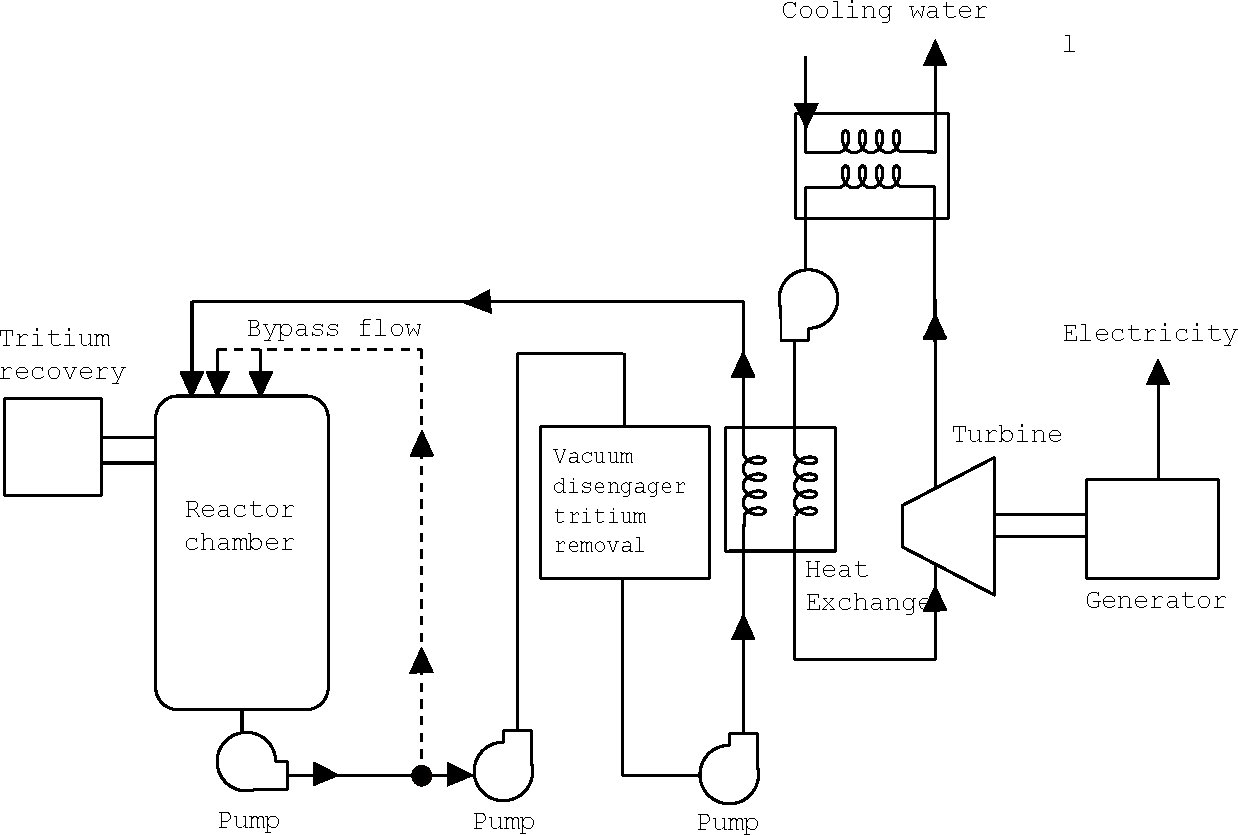
\includegraphics[width=0.8\linewidth]{StandardFigures/steamPbLi-eps-converted-to.pdf}
\caption{Main coolant system.}
\label{fig:coola}
\end{figure} 

This concept uses Lead Lithium (PbLi) as the primary coolant, and water as the secondary coolant. 

The costs are , relative to thermal power, the primary coolant systems total 10 M USD, secondary total 16 M USD, resulting in a system cost of 26 M USD. 
\subsubsection{Cost Category 22.03: Auxiliary Cooling Systems}

The Cost Category 22.03, originally designated for auxiliary cooling, was primarily considered for cryogenic cooling systems related to magnets. It has been recommended that all cooling services, including those initially covered under Account 22.03, be directly associated with the specific account requiring those services. In this instance, the auxiliary cooling services for the magnets are to be included under Cost Category 22.02.04, which deals with Cryogenics for Plasma Confinement. Auxiliary Cooling Systems therefore currently consists of:

\begin{itemize}
    \item Cost Category 22.03.04 Power Supply and Cooling System: 
    \begin{itemize}
        \item Cost Category 22.03.04.01 Refrigeration: Systems for maintaining low temperatures in critical areas.
        \item Cost Category 22.03.04.02 Piping: Network of pipes for the distribution of cooling fluids.
        \item Cost Category 22.03.04.03 Fluid Circulation Driving System: Mechanisms for propelling cooling fluids throughout the system.
        \item Cost Category 22.03.04.04 Tanks: Storage units for cooling fluids or refrigerants.
        \item Cost Category 22.03.04.05 Purification: Processes to ensure the purity and effectiveness of cooling fluids.
    \end{itemize}
    \item Cost Category 22.03.05 Other Cooling Systems: Additional cooling systems not categorized elsewhere.
\end{itemize}

Costs are expressed as 30\% of the power supply costs to give a total of \$ 83.7 M.

\subsubsection{Cost Category 22.04: Radioactive Waste Treatment} 
In the realm of managing radioactive materials in fusion energy systems, several key processes are pivotal. Firstly, the purification of the liquid breeder or heat transfer media is essential to maintain the concentration of radioactive products, specifically Lead Lithium (PbLi), within safe limits.  Radioactive materials necessitate careful classification for either recycling, clearance, or disposal in appropriate off-site repositories.  According to El-Guebaly et al. in “Goals, Challenges, and Successes of Managing Fusion Active Materials,” \cite{Elguebaly} radioactive materials must be prepared for either recycling, clearance, or proper disposal in designated off-site repositories.  The processing equipment is likely located in the Hot Cell building. This equipment encompasses remote handling tools, storage tanks, pumps, piping, valves, heat exchangers, heaters, condensers, gas strippers, compressors, chemical reactors, evaporators, ion exchange subsystems, filters, traps, and separators.  The on-site system is designed for basic processing and management, not for extensive processing. It does not serve as the primary system for online separation of Deuterium and Tritium fuel isotopes, which is handled by the Fuel Handling and Storage system (Account 22.5). Nonetheless, cost-effectively recovered tritium, such as from detritiation processes, is reintegrated into the Fuel Handling and Storage system for further refinement.\\

Consists of: 

\begin{itemize}
\item Cost Category 22.04.01 liquid waste processing and equipment.  This involves purifying the liquid breeder or heat transfer medium,  maintaining the concentration of radioactive products, in this case Lead Lithium (PbLi), below specific safety limits.
\item Cost Category 22.04.02 gaseous wastes and off-gas processing system. It involves capturing, filtering, and treating off-gases to remove contaminants and reduce radioactive emissions. This process is vital for minimizing environmental impact and adhering to stringent safety standards.
\item Cost Category 22.04.03 solid waste processing equipment. It involves the segregation, treatment, and preparation of solid wastes for safe storage or disposal. This process is essential for ensuring long-term environmental safety and compliance with regulatory requirements.
\end{itemize}




It's important to note that fusion reactors produce less long-lived radioactive waste compared to fission reactors. The IAEA notes that fusion reactor waste is primarily composed of activated structural materials, and the volume of high-level waste is significantly less \cite{girard2008summary}. This makes waste management in fusion reactors potentially more manageable and less hazardous over the long term. The development of low-activation structural materials remains a key enabling technology for fusion implementation and public acceptance.\\

Costs are scaled relative linearly with neutron power. The resultant total cost is \$ 11.313102078260872 M. Referencing Table D.1. PWR-12 cost breakdown using the GIF/EMWG COA from `A Joint Report by the OECD Nuclear Energy Agency and the International Atomic Energy Agency Measuring Employment Generated by the Nuclear Power Sector'  OECD 2018 NEA No. 7204 NUCLEAR ENERGY AGENCY.

\subsubsection{Cost Category 22.05: Fuel Handling and Storage}

The fuel handling and storage system in fusion reactors is responsible for the online processing of fuel isotopes, encompassing extraction, recovery, purification, preparation, and storage. Separate from fuel injection, this system processes materials from various sources including liquid breeders, chamber gases, and tritium-bearing streams, ensuring safe tritium levels in power core and heat transfer fluids under normal and emergency conditions.  \\

While most equipment is commercially available, heightened reliability and integrity standards, especially for tritium-containing materials, lead to higher costs. For example, atmospheric tritium recovery systems are costly due to the need for rapid and efficient tritium concentration reduction. This account's functionality and requirements are well-understood from existing and developing fusion facilities, with revisions from previous versions. Cost increases are expected due to higher reliability demands for power plant applications, but this may be offset by learning curve effects in subsequent plant constructions. The recommended Life-Cycle Analysis (LSA) factors for all accounts are 0.85 (LSA1) and 0.94 (LSA 2), reflecting these considerations.\\

  Consists of: 

\begin{itemize}
\item Cost Category 22.05.01 Chamber exhaust gas handling and processing equipment (H\&P).  Equipment for filtering, treating, and safely managing exhaust gases from the reactor chamber.
\item Cost Category 22.05.02 Purge and cover gas H\&P. Systems used for handling and processing gases that protect fuel and reactor components from contamination.
\item Cost Category 22.05.03 Primary coolant stream H\&P. Equipment involved in the handling and processing of the primary coolant stream, essential for maintaining coolant integrity.
\item Cost Category 22.05.04 Purification and isotope separation. Systems for the purification of reactor materials and the separation of isotopes, vital for fuel quality and waste management.
\item Cost Category 22.05.05 Tritium, deuterium and DT storage. Facilities for storing tritium, deuterium, and DT mixtures, which are integral to nuclear fusion reactions. 
\item Cost Category 22.05.06 Atmospheric tritium recovery. Systems designed to recover tritium from the atmosphere within the reactor facility, crucial for environmental protection and resource conservation
\end{itemize}

Various previous systems and cost analyses are available as extrapolation points, in particular For this report, ITER is used as the benchmark, then linearly scaled by $P_E$, scaled for inflation, and a learning curve credit of 0.8 is applied, equating to a factor of 0.5 for a nth-of-a-kind system.  The resulting total cost is 88.7 M USD. A breakdown of costs for each susbsystem for ITER and this concept can be found in table \ref{tab:fuel}.



\begin{table}
    \centering
    \begin{tabular}{lcc}
    \hline
        Cost Category & ITER Costs (M USD) & Scaled Costs (M USD)\\
        \hline
       22.05.01  & 29.3 & 13.9\\
       22.05.02  & 10.0 & 4.8\\
       22.05.03  & 32.2 & 15.3\\
       22.05.04  & 14.0 & 6.7\\
       22.05.05  & 32.6 & 15.6\\
       22.05.06  & 68.0 & 32.4\\
       22.05.00  & 186.0   & 88.7\\
       \hline
    \end{tabular}
    \caption{Breakdown of fuel handling and storage subsystems for ITER and the concept presented in this report.}
    \label{tab:fuel}
\end{table}

\subsubsection{Cost Category 22.06: Other Heat Island Equipment}

This Cost Category encompasses various essential components and systems of a reactor plant that are not specifically categorized elsewhere. This category is crucial for the comprehensive coverage of all necessary equipment in reactor plant operations and maintenance, safety and compliance.  This category includes, but is not limited to:


\begin{itemize}
    \item Cost Category 22.06.01 Maintenance Equipment
    \item Cost Category 22.06.01.01 Blanket Maintenance Equipment. Tools and systems for maintaining the blanket.
    \item Cost Category 22.06.01.02 Components Rotated into Service. Spare components used to replace operational ones during maintenance.
    \item Cost Category 22.06.01.03 Other. Miscellaneous equipment required for general maintenance activities.
    \item Cost Category 22.06.02 Special Heating Systems
    \item Cost Category 22.06.02.01 Start-up Systems. Equipment used for heating processes during start-up phases.
    \item Cost Category 22.06.03 Coolant Receiving, Storage and Make-up Systems.
    \item Cost Category 22.06.03.01 Coolant Handling. Systems for receiving, storing, and preparing coolant.
    \item Cost Category 22.06.04 Gas Systems
    \item Cost Category 22.06.04.01 Gas Handling and Management. Systems for managing gases used in or produced in the Heat Island.
    \item Cost Category 22.06.05 Building Vacuum Systems.
    \item Cost Category 22.06.05.01 Vacuum Maintenance. Systems to maintain vacuum conditions within certain Heat Island areas, crucial for operational integrity and safety.
\end{itemize}

Due to the broad nature of this cost category, bottom-up calculations are difficult to perform, without precise details and engineering designs. For costing purposes, we allocate 10\% of the cost of cost category 22.1 Heat Island component costs to this category, and the total budget is 1 M USD.
\subsubsection{Cost Category 22.07: Instrumentation and Control }

For a NOAK plant, it is anticipated that the I\&C technologies will be much more advanced than current  capabilities. This system will include the power core instrumentation and control, radiation and  monitoring equipment, isolated indicating and recording equipment, data acquisition and  recording, communication equipment, benchboards, panels, racks, process computers, I\&C tubing and fittings, instrumentation, and software, consisting of the following cost items:

\begin{itemize}
\item Cost Category 22.07.01 Heat Island Instrumentation and Control Equipment. Instrumentation and control equipment to monitor and manage the plasma and all  its related functional equipment contained in the Heat Island (includes all equipment in Account 22).

\item Cost Category 22.07.02 Radiation Monitoring Equipment. Monitoring equipment to ensure safe levels of radiation are maintained  during routine plant operations, determining the tritium inventories in all plant components, and  analyze/report any fault or accidental release of radioactive materials. 

\item Cost Category 22.07.03 Steam Turbine Control Equipment	

\item Cost Category 22.07.04 Other Major Component Control Equipment	

\item Cost Category 22.07.05 Signal Processing Equipment	

\item Cost Category 22.07.06 Control Boards, Panels, \& Racks	
\item Cost Category 22.07.07 Distributed Control System Equipment	
\item Cost Category 22.07.08 Instrument Wiring and Tubing	
\item Cost Category 22.07.09 Other Instrumentation \& Controls Equipment	


\end{itemize}


We use the NETL Case B31A Category 12 Instrumentation and Control for a 727MW Net power plant with bare erected costs of \$14M representing 19\$/kW.  Instrumentation in the heat island remains a major cost driver for FOAK, but by NOAK should come pre-packaged as multiple instrument packages, totalling \$ 50M, giving 88\$/kW.   We calculate \$ 85 M for this cost category.
\subsection{Cost Category 23: Turbine Plant Equipment}

\begin{figure}[h!]   
\centering   
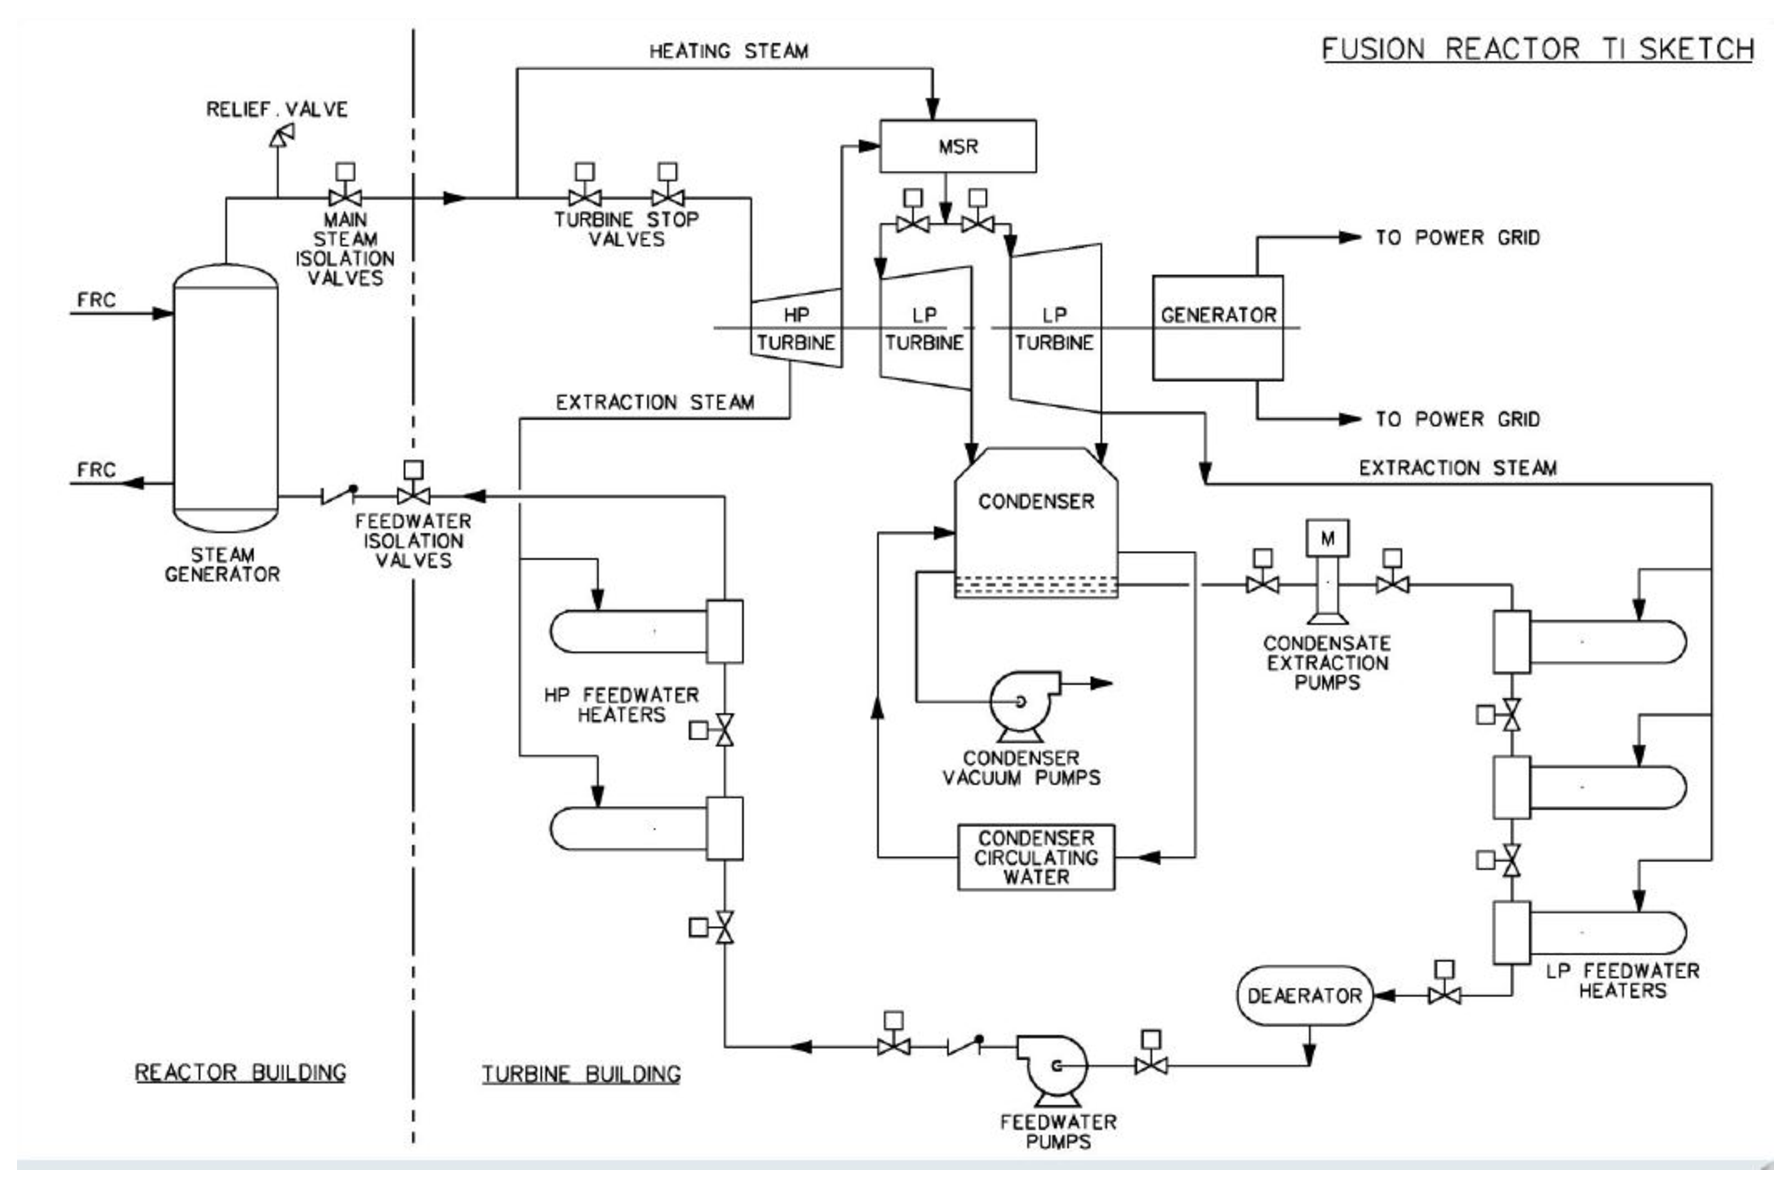
\includegraphics[scale=0.5]{StandardFigures/TIsketch.eps}   
\caption{Turbine island, per the 2017 ARPA-E study \cite{Bechtel2017}.}   
\label{fig:ti}   
\end{figure}   

Turbine Generator Equipment: This category assumes that electricity is the primary product. The categories below apply mostly to a steam-driven turbine; however, similar categories would exist for gas-driven turbines. This account includes all process equipment and systems associated with the plant output.

\begin{itemize}
    \item Cost Category 23.10.00 Turbine Generator(s): Includes turbine generator plus associated mountings, main steam control and isolation valves, lubrication system, gas systems, moisture separator, and drain system, excitation system, and controls. Main steam piping is in Account 22.20.00.
    \item Cost Category 23.30.00 Condensing Systems: Includes condenser equipment, the condensate system, the gas removal system, the turbine bypass system, condenser-cleaning system, and piping from condenser to the feedwater heating system (Cost Category 23.40.00). Condensate polishing is in Account 23.50.00
    \item Cost Category 23.30.00 Feed Heating Systems: Includes the feed heating system, feedwater heaters, feedwater system piping, the extraction steam system, and the feedwater heater vent and drain system. Piping to the steam generator continues with Cost Category 22.20.00.
    \item Cost Category 23.50.00 Other Turbine Plant Equipment: Includes piping system, turbine auxiliaries, closed cooling water system, demineralized water make-up system, chemical treatment system, and neutralization system. The cooling towers are in Cost Category 26.00.00.
    \item Cost Category 23.60.00 Instrumentation and Control (I\&C): Includes turbine generator control equipment, process computer, and BOP I\&C, including software, tubing, and fittings. Cables are in Cost Category 24.6.
    \item Cost Category 23.70.00 Turbine Plant Miscellaneous Items: Includes painting, welder qualification, and turbine plant insulation.
\end{itemize}

Cost basis is NETL baseline Case B12A, Cost Category 8: Steam Turbine and Accessories Bare erected cost excluding engineering, construction management, and contingency \$150 million in source table for Coal Plant / 686 MW electric capacity in source table = \$219/kW applied to gross thermal power, to give a total of \$ 59 M.

\subsection{Cost Category 24: Electric Plant Equipment}

Consists of the switchgear, station service eqiupment, switchboards, protective equipment, electrical structures and wiring containers, power and control wiring and electrical lighting.  Accounts 21 through 23 all have interfaces with the power plant electrical service system and its associated equipment. This equipment is located both inside and outside the main reactor/BOP buildings.

\begin{itemize}

\item Cost Category 24.01.00 Switchgear: Includes switchgear for the generator and station service, generator transformer, auxiliary transformer, and connecting bus (typically to 10kV).

\item  Cost Category 24.02.00 Station Service Equipment: Includes substations, auxiliary power sources, load centers, motor control centers, and station service and startup equipment, transformers, and bus ducts (typically to 500V).

\item  Cost Category 24.03.00 Switchboards: Includes control panels, auxiliary power and signal boards, batteries, DC equipment, and non-uninterruptible power.

\item  Cost Category 24.04.00 Protective Systems Equipment: Includes grounding systems, lightning protection, cathodic protection, heat tracing, freeze protection equipment, radiation monitoring, environmental monitoring equipment, raceway, cable, and connections. Excludes communication systems and building services such as lighting, HVAC, and fire protection (which are included in their respective building accounts).

\item  Cost Category 24.05.00 Electrical Raceway Systems: Includes cable tray, exposed conduits, embedded conduits, underground conduit and duct systems, and the fittings, supports, covers, boxes, access holes, ducts, and accessories for the scheduled cable systems. Excludes raceways for protective systems (Account 24.4) and building services electrical systems (which are included in their respective building
accounts).

\item  Cost Category 24.06.00 Power and Control Cables and Wiring: Typically includes all scheduled cable systems and their associated fittings such as cable, straps, attachments, terminations, wire lugs, cable numbers, and wire numbers. Excludes lighting, communication, and other protection systems.

\end{itemize}

Cost basis is the NETL baseline Case B12A, Cost Category 11: Accessory Electric Plant Bare erected cost excluding engineering, construction management, and contingency \$37 million in source table for Coal Plant / 686 MW electric capacity in source table = \$54/kW applied to gross  thermal power, to give a total of \$ 15 M.
\subsection{Cost Category 25: Miscellaneous Plant Equipment}  %is 26 in the geniv2007

Consists of items not in the other cost categories.

\begin{itemize}

\item Cost Category 25.01.00 Transportation and Lift Equipment: Includes cranes and hoists. (Elevators are in their respective building accounts.)

\item  Cost Category 25.02.00 Air, Water, Plant Fuel Oil, and Steam Service Systems

\item  Cost Category 25.03.00 Communications Equipment: Includes telephones, radio, CCTV, strobe, public address, enunciator, and electronic access control and security systems.

\item  Cost Category 25.04.00 Furnishing and Fixtures: Includes safety equipment, chemical laboratory equipment, instrument shop equipment, maintenance shop equipment, office equipment and furnishings, change room, and dining facility equipment.

\end{itemize}

Costs are scaled relative to thermal power, with factor 0.038\$/MW, to give a total of \$ 10 M. 

\subsection{Cost Category 26: Heat Rejection} 

This cost scales primarily with the difference between the thermal power and the gross electric power (heat rejection). Scales per Delene as overall system with spares allowance.  Subsystems include water intake, circulating water systems, cooling towers, and other systems which reject heat to the atmosphere. The cooling towers provide the ultimate heat sink for the condenser cooling and service water systems.  For this cost study, the cooling towers are assumed to be mechanical draft (fans) rectangular cell-type towers.  On-site power (standby power) will be available to sustain operation of the plant following a loss of off-site power. The site is assumed to be located near a surface water source for makeup water needs of the plant.  The power plant is assumed to be located in a warm/humid climate at a nominal plant elevation of 100 feet above sea level.  

\begin{itemize}
    \item Cost Category 26.01.00 Structures: Includes structures for the make-up water and intake, the circulating water-pump house, the make-up water pre-treatment building, and the cooling towers.
    \item Cost Category 26.02.00 Mechanical Equipment: Includes the heat rejection mechanical equipment such as circulating water pumps, piping, valves, mechanical draft cooling towers, water treatment plant, intake water pumps, screens, and filters. Excludes condensers and natural draft towers.
\end{itemize}

Cost basis: NETL baseline NGCC costs. Exhibit 5-7, Cost Category 9: Cooling System. Bare erected cost excluding engineering, construction mgmt, and contingency \$28 million in source table for NGCC / 263 MW electric capacity in source table for NGCC = \$107/kW to give a total of 7 M USD.









\subsection{Cost Category 27: Special Materials}

This account contains the costs of specific types of materials that are introduced into the fusion power plant immediately before the initiation of testing and validation procedures. These materials are characterized within conventional categories, encompassing coolants, cover gases designed for material handling systems and architectural components, breathable air containing specific compositions, as well as gases or liquids that have not been pre-loaded into the existing plant systems. It is essential to classify these materials as intrinsic components of the capital equipment, distinct from the diverse plant systems, and therefore not subject to acquisition via construction loans. The replenishment process for  these materials is to be delineated as an operational expense. Among the specialized materials encompassed are eutectic salts, treated water, liquid metals,  cryogenic liquids, gases with unique properties, and potentially select solid materials, moderator and/or reflector materials that are non-fuel and non-structural in nature. Special heat transfer fluids, which are different from natural water, and may be in the form of gases or liquids. This includes primary and secondary coolant, intermediate loop heat transport fluid, and turbine cycle working fluids. The initial supply of oil, lubricants, ion exchange resins, boric acid, and gases such as $N_2$, $O_2$, He, and $CO_2$.
This category is further broken down into sub-categories:

\begin{itemize}
    \item Cost Category 27.01.00 Primary Coolant. Costs are based on volumes. For a primary coolant of primaryC with a volume of primaryV cubic meters, a cost of \$ C270100 M is obtained.  
    \item Cost Category 27.02.00 Secondary Coolant. Costs are based on volumes. For a primary coolant of secondaryC with a volume of secondaryV cubic meters, a cost of \$ C270200 M is obtained.
    \item Cost Category 27.03.00 Neutron multiplier material.  Costs are based on volumes, determined in the radial build, and a cost of \$ C270300 M is obtained.
    \item Cost Category 27.04.00   
    \item Cost Category 27.05.00 Turbine cycle working fluid.
    \item Cost Category 27.06.00 Initial materials, including oil, lubricants, resins for ion exchanger, and boric acid.
\end{itemize}

Note that for natural lithium, there is a cost per tonne quoted in the materials look-up table, Table \ref{tab:materials}.  If the lithium needs to be enriched or purified, the costs do not scale linearly with purity (since higher purity requires multiple passes through the same system).  We include a scaling with the purity therefore as the following table suggests:

\begin{table}[]
    \centering
    \begin{tabular}{c|c}
       Purity  &  Cost factor \\
       90 \%  &  1 \\
       99 \%  &  2 \\
       99.9 \%  &  4 \\
       99.99 \%  &  8 \\
       99.999 \%  &  16 \\
    \end{tabular}
    \caption{Purity cost factors}
    \label{tab:my_label}
\end{table}

Total costs for special materials is the summation over all the sub categories, giving \$ 2 M.  




\subsection{Cost Category 28: Digital twin / Simulator }

Simulator(s): This account includes the development of new digital twins or simulators.  Digital twins play a pivotal role in enhancing the safety, efficiency, and overall operational effectiveness of nuclear power plants. By creating real-time, high-fidelity digital replicas of these complex facilities, operators can continuously monitor and simulate plant behavior, predict potential issues, and optimize maintenance schedules. This technology enables proactive decision-making, reduces downtime, and ensures compliance with stringent safety standards, ultimately contributing to the reliable and sustainable 
operation of nuclear power plants.\\

Cost basis is the estimated annual license fee of 5 M USD for a comprehensive digital twin platform for the fusion power plant, based on quotes from nTtau Digital LTD.

\subsection{Cost Category 29: Contingency on Direct Capital Costs}

This account includes the assessment of additional cost that might be necessary to achieve the desired confidence level for the direct costs not to be exceeded. Contingency is usually applied at an aggregated level, although its determination may include applying contingencies to individual high-cost-impact items in the estimate.  Contingency factors range from 1 to 0.05 depending on the maturity of the subsystem, so for a FOAK Fusion Pilot Plant, the factor may be as high as 1 for all of the major subsystems included in the fusion power core, but closer to 0.05 for systems in the Balance of Plant.  \\

Here we apply a factor of 0.1 to all of the systems in Cost Category 20, giving a total of  1562603 M. {\color{blue} However for NOAK, we omit this cost.}


\section{Cost Category 30: Capitalized Indirect Service Costs (CISC)}





\subsection*{Cost Category 31 – Field Indirect Costs}
This Cost Category includes cost of construction equipment rental or purchase, temporary buildings, shops, laydown areas, parking areas, tools, supplies, consumables, utilities, temporary construction, warehousing, and other support services. Cost Category 31 also includes:

\begin{itemize}
    \item Temporary construction facilities, such as site offices, warehouses, shops, trailers, portable offices, portable restroom facilities, temporary worker housing, and tents.
    \item Tools and heavy equipment used by craft workers and rented equipment such as cranes, bulldozers, graders, and welders. Typically, equipment with values of less than \$1,000 are categorized as tools.
    \item Transport vehicles rented or allocated to the project, such as fuel trucks, flatbed trucks, large trucks, cement mixers, tanker trucks, official automobiles, buses, vans, and light trucks.
    \item Expendable supplies, consumables, and safety equipment.
    \item Cost of utilities, office furnishings, office equipment, office supplies, radio communications, mail service, phone service, and construction insurance.
    \item Construction support services, temporary installations, warehousing, material handling, site cleanup, water delivery, road and parking area maintenance, weather protection and repairs, snow clearing, and maintenance of tools and equipment.
\end{itemize}

Previously calculated as 6 percent of total direct costs based on Field Office Engineering and 
Services Table 3.2-VII of \cite{SCH78}.  Min \$130/kW, Average \$158/kW, Max \$192/kW, to give a total of \$ 370 M for a construction time of 3 years. Reduction strategies: Same as strategies listed above for construction services and  materials (91) and home office engineering and services (92).\\

Bottoms up example: 10 engineers and managers on average during construction period, with 2000 hours of work annually per engineer and manager = 60,000 man-hours of work \$150/hour average rate = \$3 million, with 150 MW for plant capacity = \$0.02/W/annum, giving total cost of \$ 6 M for a construction time of 3 years.


\subsection*{Cost Category 32 – Construction Supervision}
This Cost Category covers the direct supervision of construction (craft-performed) activities by the construction contractors or direct-hire craft labor by the A/E contractor. The costs of the craft laborers themselves are covered in the labor-hours component of the direct cost in Cost Categorys 21 through 28 or in Cost Category 31. This Cost Category covers work done at the site in what are usually temporary or rented facilities. It includes non-manual supervisory staff, such as field engineers and superintendents. Other non-manual field staff are included with Cost Category 38, PM/CM Services Onsite.\\

This cost category supersedes the Pre 2007 indirect cost categories 91 Construction Service and Materials  \\

\emph{Previous values: } 
12\% of total direct costs based on Schulte et al. (1978) and LSA of 2, giving a total of 6 M USD. Min \$261/kW, Average \$316/kW, Max \$384/kW. \\

Here we estimate from the bottoms up: 25 managers on average during construction period. 2000 hours of work annually per engineer and manager = 50,000 man-hours of work per annum \$150/hour average rate=\$7.5 million for a 150 MW plant capacity = \$0.05/W/annum, to give a total of 14 M USD for a construction time of 3 years.

\subsection*{Cost Category 33 – Commissioning and Start-up Costs}
This Cost Category includes costs incurred by the A/E, reactor vendor, other equipment vendors, and owner or owner’s representative for startup of the plant including:
\begin{itemize}
    \item Startup procedure development
    \item Trial test run services (Cost Category 37 in the IAEA Account system)
    \item Commissioning materials, consumables, tools, and equipment (Cost Category 39 in the IAEA Account system)
\end{itemize}
The utility’s (owner’s) pre-commissioning costs are covered elsewhere in the TCIC sum as a capitalized owner’s cost (Cost Category 40).

\subsection*{Cost Category 34 – Demonstration Test Run}
This Cost Category includes all services necessary to operate the plant to demonstrate plant performance values and durations, including operations labor, consumables, spares, and supplies.

\subsection*{Cost Category 35 – Design Services Offsite}
This Cost Category covers engineering, design, and layout work conducted at the A/E home office and the equipment/reactor vendor’s home office. Often pre-construction design is included here. These guidelines use the IAEA format for a standard plant (and equipment) design/construction/startup only and not the FOAK design and certification effort. (FOAK work is in the one-time deployment phase of the project and not included in the standard plant direct costs.) Design of the initial full size (FOAK) reactor, which will encompass multiple designs at several levels (pre-conceptual, conceptual, preliminary, etc.), will be a category of its own under FOAK cost. This Cost Category also includes site-related engineering and engineering effort (project engineering) required during construction of particular systems, which recur for all plants, and quality assurance costs related to design.\\

Previously this was Cost Category 92 - Home Office Engineering Services.  Home Office Engineering and Services  Table 3.2-VII of \cite{SCH78}.\\

Adaptations to generic plant design for the specific construction project by off-site engineers, and other necessary off-site engineering support. Note: In this standard framework for nuclear plant cost accounting, only activities for specific construction projects at particular sites should be included in this code or any other. Initial work by plant vendors to design their generic concepts and license them with the NRC should be excluded from project-specific cost accounting. Plant vendors can recover their initial design and licensing costs over several projects (e.g., first through fifth) by applying an adder, perhaps as part of overhead for profitability, to the project-specific costs.\\


5\% of total direct costs based on Schulte et al. (1978). Min \$113/kW, Average \$137/kW, Max 
\$166/kW, to give a total of 320 M USD.  Reduction strategy includes standardized and reusable plant design; avoidance of regulatory or 
plant owner modifications to generic design.\\


Example basis: 15 engineers and managers on average during construction period. 
1000 hours of work annually per engineer and manager = 30,000 man-hours of work per 
annum at \$150/hour average rate = \$4.5 million per annum with 150 MW for plant capacity $=$ \$0.03/W/annum and a total of 9 M for a construction time of 3 years. 


\subsection*{Cost Category 36 – PM/CM Services Offsite}
This Cost Category covers the costs for project management and construction management support on the above activities (Cost Category 31) taking place at the reactor vendor, equipment supplier, and A/E home offices.

\subsection*{Cost Category 37 – Design Services Onsite}
This Cost Category includes the same items as in Cost Category 35, except that they are conducted at the plant site office or onsite temporary facilities instead of at an offsite office. This Cost Category also includes additional services such as purchasing and clerical services.

\subsection*{Cost Category 38 – PM/CM Services Onsite}
This Cost Category covers the costs for project management and construction management support on the above activities taking place at the plant site. It includes staff for quality assurance, office administration, procurement, contract administration, human resources, labor relations, project control, and medical and safety-related activities. Costs for craft supervisory personnel are included in Cost Category 32.

\subsection*{Cost Category 39 – Contingency on Support Services}
This Cost Category includes an assessment of additional cost necessary to achieve the desired confidence level for the support service costs not to be exceeded.


\section{Cost Category 40: Capitalized Owner’s Cost (COC)}

Previously was Cost Category 94 and was calculated as 23 \% of total direct costs based on Owner's Cost - Table 3.2-VII of \cite{SCH78} and LSA of 2. Costs of \$ 386 M are estimated. Reduction strategies include streamlined processes for staff recruitment etc. 

\subsection*{Cost Category 41 – Staff Recruitment and Training}
This Cost Category includes costs to recruit and train plant operators before plant startup or commissioning activities (Cost Category 33), or demonstration tests (Cost Category 34).

\subsection*{Cost Category 42 – Staff Housing}
This Cost Category includes relocation costs, camps, or permanent housing provided to permanent plant operations and maintenance staff.

\subsection*{Cost Category 43 – Staff Salary-Related Costs}
This Cost Category includes taxes, insurance, fringes, benefits, and any other salary-related costs.

\subsection*{Cost Category 44 – Other Owner’s Costs}

\subsection*{Cost Category 49 – Contingency on Owner’s Costs}
This Cost Category includes an assessment of additional costs necessary to achieve the desired confidence level for the capitalized owner’s costs not to be exceeded.

\section{Cost Category 50: Capitalized Supplementary Costs (CSC)}


\subsection*{Cost Category 51 – Shipping and Transportation Costs}
This Cost Category includes shipping and transportation costs for major equipment or bulk shipments with freight forwarding. Budget is \$ 8 M.

\subsection*{Cost Category 52 – Spare Parts}
This Cost Category includes spare parts furnished by system suppliers for the first year of commercial operation. It excludes spare parts required for plant commissioning, startup, or the demonstration run.  Budget is \$ 24 M, which is calculated on the basis of 10 \% of the direct cost components in the BOP (note that Scheduled Replacement Costs for the heat island are calculated in Cost Category 75.

\subsection*{Cost Category 53 – Taxes}
This Cost Category includes taxes associated with the permanent plant, such as property tax, to be capitalized with the plant. Budget is \$ 100 M.

\subsection*{Cost Category 54 – Insurance}
This Cost Category includes insurance costs associated with the permanent plant to be capitalized with the plant.  Budget is \$ 1 M.

\subsection*{Cost Category 55 – Initial Fuel Load}
This Cost Category covers fuel purchased by the utility before commissioning, which is assumed to be part of the TCIC. For DT systems this will include the initial tritium startup costs.  Due to its scarcity, tritium costs \$109,570 to \$169,570 per gram in 2016 USD. Therefore, the onetime start-up tritium cost ranges from \$22 M to \$34 M (2016 USD) for a standard 150 MWe FPP. \\

We allocate a budget of \$ 41 M for the initial fuel load.  

\subsection*{Cost Category 58 – Decommissioning Costs}
This Cost Category includes the cost to decommission, decontaminate, and dismantle the plant at the end of commercial operation, if it is capitalized with the plant.  This cost used to be broken out as a separate line item in the cost of electricity calculation.\\

The D\&D allowance are assumed flat and constant for the systems under consideration here, and we base the amount on the following:

\begin{verbatim} 
Decontamination and Decommissioning Allowance 
TFTR (51 MWth) $36.7M (Actual 2002$) 
Generic Magnetic Fusion Reactor 0.5 M/kWh (1983$) 
Light Water Reactor $307M - $819M (Actual 2013$) 
Generic Magnetic Fusion Reactor Revisited, J Sheffield/S Milora,  
ANS Fusion Science and Technology Vol.70, 14-35, July 2016. 
Decommissioning of the Tokamak Fusion Test Reactor,
Perry/Chrzanowski/Gentile/Parsells/Rule/Strykowsky/Viola, 
Princeton Plasma Physics Laboratory, PPPL-3895, October 2003.
Costs of Decommissioning Nuclear Power Plants, NEA No. 7201. OECD 2016.
\end{verbatim} 

Prior to 2007, these costs were included in the LCOE as a budget of 0.5mills/kWh.  Here, we provide a budget estimate for the decommissioning costs of \$ 200 M.  

\subsection*{Cost Category 59 – Contingency on Supplementary Costs}
This Cost Category includes an assessment of additional cost necessary to achieve a desired confidence level for the capitalized supplementary costs not to be exceeded. The contingency for the initial core load should not be applied to this item, because the contingency is already embedded in the fuel cycle costs from the fuel cycle model.\\

Budget is \$ 0 M, based on 10 \% of the sum of the CSC.

\section{Cost Category 60: Capitalized Financial Costs (CFC)}

\subsection*{Cost Category 61 – Escalation}
This Cost Category is typically excluded for a fixed year, constant dollar cost estimate, although it could be included in a business plan, a financing proposal, or regulatory-related documents.  Formerly Cost Category 98 pre 2007.\\

Escalation during Construction (EDC), which results from increases (or decreases) in the costs of labour 
or materials due to inflation (or recession and deflation). Table 3.2-X of \cite{SCH78}, to give a total of \$ 60 M.

\subsection*{Cost Category 62 – Fees}
This Cost Category includes any fees or royalties that are to be capitalized with the plant.\\

Fees or royalties are not included.

\subsection*{Cost Category 63 – Interest During Construction (IDC)}
This Cost Category is discussed in Chapter 7 of the G4EMWG guidelines. IDC is applied to the sum of all up-front costs (i.e., Cost Category 10 through 50 base costs), including respective contingencies. These costs are incurred before commercial operation and are assumed to be financed by a construction loan. The IDC represents the cost of the construction loan (e.g., its interest). Formerly Cost Category 97 (pre 2007).\\

Compound interest on debt and rate of return on equity investments during construction 
period depends on weighted average cost of capital between interest rate and equity  return as well as construction duration for compounding calculation. Previously,  49 percent of total direct costs based on Interest during Construction (IDC) Table 3.2-X of \cite{SCH78}.  Total based on LSA of 2 was \$ 1791 M. Min \$1,075/kW, Average \$1,302/kW, Max \$1,582/kW. Reduction strategies can include minimizing interest rate and equity return: Government financing or loan guarantees; minimal project risk to assure lenders and equity investors. Minimize construction duration:  Streamlined planning and processes; completed designs before construction starts and no subsequent  changes; minimal construction project risks to avoid rework and delays.\\

Calculated here: 7 percent weighted average cost of capital = 10 percent added for interest during 
construction (approximate calculation - accounts for spreading construction expenditures across construction time) \$99/kW. Total cost here is 18 M USD.

\subsection*{Cost Category 69 – Contingency on Capitalized Financial Costs}
This Cost Category includes an assessment of additional cost necessary to achieve the desired confidence level for capitalized financial costs not to be exceeded, including schedule uncertainties.\\

Currently not calculated.




\subsection{Cost Category 70: Annualized O\&M Cost (AOC)}

The Operations and Maintenance (O\&M) costs was previously estimated to be 2 \% of the direct cost, assessed annually.  The O\&M cost depends on the system complexity and the requirements of regulations, security and maintenance. The costs are computed based on look-up tables, such as the one shown in Fig. \ref{fig:statista} at 60 USD per kilowatt-year.  

\begin{figure}[b!] 
\centering 
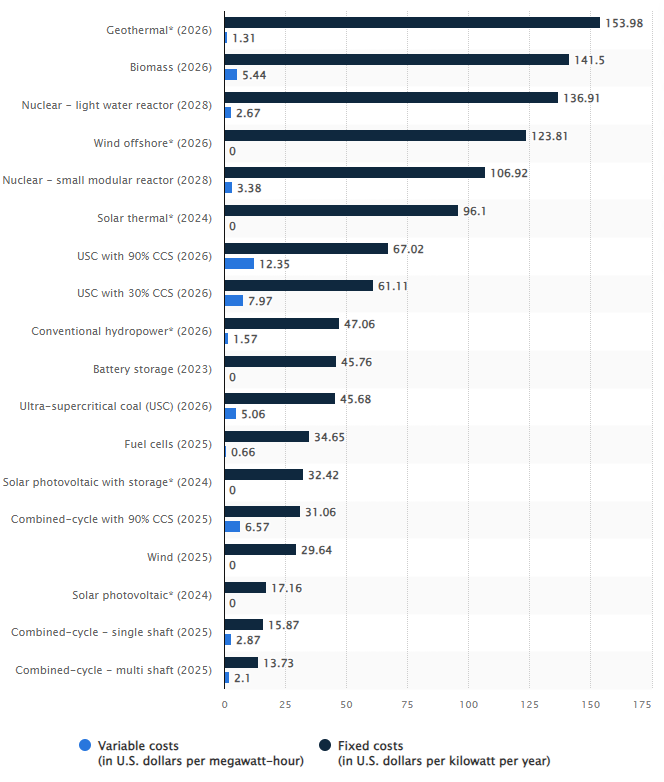
\includegraphics[scale=0.5]{StandardFigures/statista.png} 
\caption{Operations and Maintenance costs for various kinds of power plants.} 
\label{fig:statista} 
\end{figure} 

\begin{verbatim} 
C_OM = 60 * PE * 1000 = 4  
\end{verbatim} 

Annualized O\&M costs are \$ 4 M.

\subsubsection*{Cost Category 71 – O\&M Staff}
Component in the financial structuring of operational expenditures in various industries, especially those involving significant infrastructure and machinery, such as power generation, manufacturing, and utilities.  The costs under Cost Category 71 predominantly include:

\begin{itemize}
    \item \textbf{Salaries:} The regular wages paid to the O\&M staff.
    \item \textbf{Training and Development:} Costs associated with professional development, training programs, and certifications to ensure staff is up-to-date with the latest operational and maintenance practices.
    \item \textbf{Overtime and Shift Allowances:} Compensation for extended work hours and shift differentials, especially in 24/7 operational setups.
\end{itemize}

Cost Category 71 is crucial in operational budgeting due to:

\begin{enumerate}
    \item \textbf{Staffing Optimization:} The need for an optimal number of skilled staff to ensure efficient and safe operations.
    \item \textbf{Direct Impact on Operational Efficiency:} The performance and availability of O\&M staff directly affect operational uptime and efficiency.
    \item \textbf{Regulatory Compliance:} Compliance with labor laws and industry-specific regulations regarding staffing and worker safety.
\end{enumerate}

\textit{Cost Category 71 – O\&M Staff} encompasses all aspects of costs related to the personnel responsible for the operation and maintenance of facilities. Efficient management of this category is vital for ensuring operational excellence, staff well-being, and overall financial health of the organization.


\subsubsection*{Cost Category 72 – Management Staff}
Crucial aspect of operational expenses in various sectors, especially in industries where effective management plays a pivotal role in ensuring efficient operations and achieving organizational objectives.  Cost Category 72 typically encompasses:

\begin{itemize}
    \item \textbf{Salaries:} The basic remuneration paid to operations management staff.
    \item \textbf{Bonuses and Incentives:} Performance-related bonuses and incentives that align management objectives with corporate goals.
    \item \textbf{Professional Development:} Expenses related to the continuous learning and development of management skills, including workshops, seminars, and courses.
    \item \textbf{Leadership Training:} Specific training focused on enhancing leadership qualities necessary for effective management.
\end{itemize}

The inclusion of Cost Category 72 in operational expenditure is significant due to:

\begin{enumerate}
    \item \textbf{Strategic Decision Making:} Management staff play a crucial role in strategic decision-making and operational planning.
    \item \textbf{Operational Efficiency:} Effective management is key to ensuring operational efficiency and organizational success.
    \item \textbf{Staff Leadership:} Management staff are responsible for leading, guiding, and motivating the workforce, directly impacting productivity and morale.
\end{enumerate}

\textit{Cost Category 72 – Management Staff} is integral to the financial planning of any organization, particularly in operational contexts. It involves not just the direct costs of salaries and benefits but also the broader implications of effective management on organizational performance and success.

\subsubsection*{Cost Category 73 – Salary-Related Costs}
This Cost Category includes taxes, insurance, fringes, benefits, and any other annual salary-related costs.

\subsubsection*{Cost Category 74 – Operations Chemicals, and Lubricants}

\subsubsection*{Cost Category 75 – Spare Parts}
Critical element in the operational budgeting of various industries, particularly in sectors that rely on continuous and efficient machinery and equipment operation.  This cost category encompasses:

\begin{itemize}
    \item \textbf{Operational Spare Parts:} Expenses associated with spare parts used in regular operations. These do not include major equipment or capital plant upgrades.
    \item \textbf{Exclusion of Capitalized Items:} It specifically excludes items that would be capitalized or amortized over a period or quantity of product.
\end{itemize}

Cost Category 75 plays a significant role in Operations and Maintenance (O\&M) budgeting, as it:

\begin{itemize}
    \item \textbf{Ensures Operational Continuity:} Regular replacement and availability of spare parts are crucial for uninterrupted operations.
    \item \textbf{Impacts Maintenance Scheduling:} Influences the planning and scheduling of maintenance activities.
    \item \textbf{Affects Operational Efficiency:} Directly impacts the overall efficiency and lifespan of the operational equipment.
\end{itemize}

\textit{Cost Category 75 – Spare Parts} is essential for the smooth operation and maintenance of machinery and equipment in various industries. It encompasses the costs of spare parts necessary for regular operation and scheduled component replacements, playing a vital role in operational budgeting and efficiency.  Cost of any operational spare parts, excluding capital plant upgrades or major equipment that will be capitalized or amortized over some period or quantity of product.

\subsubsection*{Cost Category 76 – Utilities, Supplies, and Consumables}
Cost of water, gas, electricity, tools, machinery, maintenance equipment, office supplies and similar items purchased annually.

\subsubsection*{Cost Category 77 – Capital Plant Upgrades}
Upgrades to maintain or improve plant capacity, meet future regulatory requirements or plant life extensions.

\subsubsection*{Cost Category 78 – Taxes and Insurance}
Property taxes and insurance costs, excluding salary related.

\subsubsection*{Cost Category 79 – Contingency on Annualized O\&M Costs}
This Cost Category includes an assessment of additional cost necessary to achieve the desired confidence level for the annualized O\&M costs not to be exceeded.

\subsection{Cost Category 80: Annualized Fuel Cost (AFC)}

%\subsection{Annual Fuel Cost} 
The fuel cost, C$_{F}$, is calculated as follows.  The unit cost of deuterium as D2 is 3,700 \$/kg; deuterium contributes negligibly to the COE of a fusion power plant. In the long run, the power plant is self-sufficient in terms of tritium fuel production because of the breeding capability of the blanket so that no specific tritium-fuel charge is reported. It should be recognized, however, that there is a significant cost for tritium in the direct cost of the D-T fueled fusion reactor, represented in Cost Category 22.05 Fuel Handling and Storage. Cost of the primaryC and secondaryC coolant is included in Cost Category 27 Special Materials.\\

Consists of:  
\begin{verbatim} 
m_D = 3.342*10^(-27) # (kg)
u_D = 2175 #Where u_D ($/kg) = 2175 ($/kg) 
C_F = N_mod * P_NRL * 1e6 * 3600 * 8760 * u_D * m_D * p_a / (17.58 * 1.6021e-13)
\end{verbatim} 

Total annual fuel costs are \$ 0 M per year.

\subsubsection*{Cost Category 81 – Refueling Operations}
This Cost Category includes incremental costs associated with refueling operations.

\subsubsection*{Cost Category 84 – Fuel}
This Cost Category includes annualized costs associated with the fuel cycle.

\subsubsection*{Cost Category 86 – Processing Charges}
This Cost Category includes storage and processing if fuel is brought in from offsite.

\subsubsection*{Cost Category 87 – Special Nuclear Materials}
This Cost Category covers materials such as heavy water, sodium, lead, helium, or other energy transfer mediums that are required on an annual basis. It includes costs associated with disposal or treatment if necessary. 

\subsubsection*{Cost Category 89 – Contingency on Annualized Fuel Costs}
This Cost Category includes an assessment of additional cost necessary to achieve the desired confidence level for the annualized fuel costs not to be exceeded.

\subsection{Cost Category 90: Annualized Financial Costs (AFC)}


Consists of: Capital recovery factor (or constant dollar FCR), $f_{cr}$ multiplied by the total capital cost. This is a function of the cost of money and the period over which the investment must be paid off (see 2019 NETL report \cite{NETL2019a}). In this case, it is the lifetime of the plant, plifetime years, plus the construction time, constructionTime years. Thus, the capital recovery factor is calculated from 

\begin{equation}
    C(x,N) = \frac{x(1+x)^N}{(1+x)^N-1} = \left[ \sum_{n=1}^N \frac{1}{(1+x)^N}] \right] ^{-1},
    \label{eq:C}
\end{equation}

where 

\begin{equation}
    x = i_cf_c + i_pf_p +(1-t)i_df_d
\end{equation}

is the effective cost of money. Here, $i_c$ is the rae of return on common stock, $f_c$ is the fraction of capital form common stock, $i_p$ is the rate of return of preferred stock, $f_p$ is the fraction of capital from preferred stock, $i_d$ is the nterest rate on deb, and $f_d$ is the capital from debt. 

From here, the fixed charge rate can be calculated as 
\begin{equation}
    f_{cr} = \frac{Ck}{(1-t)} - \frac{td}{(1-t)} + t_p + r,
\end{equation}

where $C$ is the capital recovery factor (\ref{eq:C}), $k$ is the adjustment for investment tax credit, $t$ is the effective income tax rate, $d$ is the levelized tax depreciation, $t_p$ is the property tax rate and $r$ is the levelized interim replacement cost. For this power plant, see \ref{tab:ec_vals} for values. Applying these calculations to this power plant with a lifetime of plifetime yields $f_{cr} = $ fcr.\\


\begin{table}
    \centering
    \begin{tabular}{cc|cc}
    \hline
      $N$ (plant life)  & plifetime & $t$ (construction period) & constructionTime\\
       $i_c$  & 0.1 & $t_p$ (property tax rate)& 0\\
        $i_p$ & 0 & $x_1$ (pre-tax)& 0.073\\
        $i_d$ & 0.05 & $x$ (post-tax)& 0.065\\
        $f_c$ & 0.45 & $x_r$ (real)& 0.045\\
        $f_p$ & 0 & $k$ & 1\\
        $f_d$ & 0.55 & $C(x,N)$ & 0.077\\
        $i$ (general inflation) & 0.02 & $C(x_r,N)$ & 0.061\\
        $e$  (escalation)& 0.02 & $r$ (interim replacement)& 0\\
        $e_r$ (real escalation) & 0 & $f$ (depreciable fraction of TCC)& 0.881\\
        $t_s$ (income tax 1) & 0.06 & $d$ (levelized depreciation)& 0.036\\
        $t_f$ (income tax 2) & 0.21 & $f_{cr}$ & 0.0910\\
        $t$ (effective income tax) & 0.257 & $f_{cr0}$ & 0.0722\\
    \hline    
    \end{tabular}
    \caption{Values used in calculation of capital recovery factor  $f_{cr}$, the effective cost of money, $x$, and the fixed charge rate, $R$.}
    \label{tab:ec_vals}
    \label{tab:my_label}
\end{table}

By multiplying the capital recovery factor, $f_{cr}$ by the total capital cost, $C_{99}$, the annual capital cost charge is calculated.
Annualized Financial Costs are \$ 445 M.

\subsubsection*{Cost Category 91 – Escalation}
Critical financial concept often used in the planning and analysis of long-term projects, particularly in industries such as energy or construction. This category accounts for the changes in costs over time due to factors like inflation, market dynamics, and changes in labor or material costs. Escalation is the systematic increase in costs over the life of a project. It is distinct from \textit{contingency}, which is used to cover unforeseen costs. Escalation accounts for known, predictable changes in cost such as:

\begin{itemize}
    \item \textbf{Inflation:} General increase in prices and fall in the purchasing value of money.
    \item \textbf{Market Fluctuations:} Changes in costs due to supply and demand dynamics.
    \item \textbf{Labor Cost Changes:} Variations in labor costs due to economic conditions or labor market changes.
    \item \textbf{Material Cost Variations:} Fluctuations in the cost of raw materials.
\end{itemize}

In many financial estimates, particularly initial cost assessments, Cost Category 91 is often excluded. This exclusion is typically because:

\begin{enumerate}
    \item \textbf{Simplification:} To simplify the early stages of financial planning.
    \item \textbf{Variability:} Due to the unpredictable nature of some escalation factors.
\end{enumerate}

While often excluded from initial estimates, escalation is crucial in:

\begin{itemize}
    \item \textbf{Business Plans:} For a realistic long-term financial outlook.
    \item \textbf{Financing Proposals:} To present a complete picture to potential investors or lenders.
    \item \textbf{Regulatory-Related Documents:} Where detailed, realistic cost projections are required.
\end{itemize}

Effective management of Cost Category 91 involves:

\begin{enumerate}
    \item \textbf{Regular Reassessment:} Continuously updating the project's cost estimates to reflect current economic conditions.
    \item \textbf{Risk Mitigation:} Developing strategies to mitigate the impact of negative cost escalations.
    \item \textbf{Informed Decision Making:} Using escalation estimates to make informed financial and strategic decisions.
\end{enumerate}



\subsubsection*{Cost Category 92 – Fees}
This Cost Category primarily encompasses the costs associated with annual fees necessary for the operation of such facilities.  Fees under Cost Category 92 typically include, but are not limited to, costs related to:

\begin{itemize}
    \item \textbf{Licensed Reactor Processes:} These are fees paid for obtaining and maintaining the licenses required for reactor operation. They cover regulatory compliance and safety standards as set by nuclear regulatory bodies.
    \item \textbf{Nuclear Operating License Fees:} Fees associated with the acquisition and renewal of operating licenses for nuclear facilities. These are critical for legal and safe operation.
    \item \textbf{Regulatory Compliance:} Fees related to ensuring compliance with various environmental, safety, and operational regulations.
    \item \textbf{Inspection and Oversight:} Costs incurred for regular inspections and oversight activities by regulatory authorities to ensure adherence to safety and operational guidelines.
\end{itemize}

\textit{Cost Category 92 – Fees} is an essential financial Cost Category, especially for nuclear facilities, where regulatory compliance and licensing play a critical role. Proper management and allocation of funds for these fees are vital for uninterrupted and legal operation.

\subsubsection*{Cost Category 93 – Cost of Money}
The \textbf{cost of money} is akin to the \textit{opportunity cost} of using capital for a specific purpose. When capital is allocated to operating costs, it is an alternative to investing that capital elsewhere. Thus, the cost of money represents the return that this capital could have earned if invested differently.
\begin{itemize}
    \item Sources of Capital. Capital for operating costs can be sourced either externally or from within the organization (retained earnings). External financing includes loans, bonds, or other forms of borrowing, incurring interest payments. Retained earnings are internal funds saved and not distributed as dividends, carrying an opportunity cost as these funds could be used elsewhere.
    \item Impact on Operating Costs. In financial Cost Categorying, the cost of money is considered an \textit{indirect cost} of operating. It reflects the financial charges incurred due to the company's capital structure, including both the direct costs (e.g., interest on loans) and the opportunity costs (e.g., using retained earnings).
    \item Project Financing and Cost of Capital.  For large-scale projects like nuclear power plants, the cost of money is crucial in project financing. The strategy (debt vs. equity) and the corresponding costs of capital significantly affect the overall project economics.
    \item Risk and Return Considerations. The cost of money reflects the project's risk profile. Higher-risk projects lead to higher costs of capital, as lenders and investors demand higher returns for increased risks.
    \item Long-term Implications.  For long-term projects, the cost of money impacts the project's \textit{net present value} (NPV) and \textit{internal rate of return} (IRR). Effective management of the cost of money is essential for the project's long-term financial viability.
    \item Dynamic Nature.  The cost of money changes with market conditions, economic environment, and the organization's financial health. This necessitates continuous monitoring and reevaluation of financing strategies.
\end{itemize}

\textbf{In summary}, Cost Category 93 - Cost of Money - encompasses the financial implications of the capital used for operating costs. It includes both direct costs (like interest payments) and indirect costs (like opportunity costs of capital). Proper management of this Cost Category is crucial for the economic feasibility and financial health of large-scale projects.




\subsubsection*{Cost Category 99 – Contingency on Annualized Financial Costs}
This Cost Category includes an assessment of additional costs necessary to achieve the desired confidence level for the annualized financial costs not to be exceeded, including schedule uncertainties. Not included here.

\newpage 
\section{Cost Accounting Structure} 

\begin{table}[h!]
\resizebox{\textwidth}{!}{
\begin{tabular}{lcccc}
\hline
& Cost (M USD) & \% of TCC & ARIES-ST Cost (M USD) & ARIES-ST \% of TCC\\
\hline
10. Pre-construction & 226 & 5 & 14.25 & 0.2091743780007396 \\
20. Direct Costs & 3214 & 74 & 74 & 30.01454989991744 \\
\hspace{5mm}21. Structures/Site & 111 & 3 & 711.93 & 5.002424983319574 \\
\hspace{5mm}22. Reactor Plant Equip. & 2626 & 61 & 4324.31 & 15.017141665902155 \\
\hspace{15mm}22.1 Reactor Equip. & 2408 & 56 & - & - \\
\hspace{15mm}22.1.1 First Wall \& Blanket & 325 & 7 & 202.92 & 1.268859670325241 \\
\hspace{15mm}22.1.2 High Temp. Shield & 38 & 1 & 213.75 & 1.3695001729482386 \\
\hspace{15mm}22.1.3 Magnets & 1436 & 33 & 1405.05 & 2.500225820065444 \\
\hspace{15mm}22.1.4 Suppl. Heating & 353 & 8 & 288.71 & 0.8110440505500376 \\
\hspace{15mm}22.1.5 Primary Structure & 57 & 1 & 155.61 & 0.5308293177565938 \\
\hspace{15mm}22.1.6 Vacuum System & 21 & 0 & 19.95 & 1.9496630704219877 \\
\hspace{15mm}22.1.7 Power Supplies & 63 & 1 & 180.69 & 1.0004849966639149 \\
\hspace{15mm}22.1.8 Electrodes or Plasma Guns & 118 & 3 & 13.40 & 0.08090707073613512 \\
\hspace{15mm}22.1.9 Direct E. Conv. & 0 & 0 & 64.98 & - \\
\hspace{15mm}22.1.11 Assembly and installation & 115 & 3 & - & - \\
\hspace{10mm}22.2 Main Heat Transfer & 39 & 1 & 674.31 & - \\
\hspace{10mm}22.3 Auxiliary Cooling & 1 & 0 & 143.07 & - \\
\hspace{10mm}22.4 Rad. Waste Treat. & 2 & 0 & 32.78 & - \\
\hspace{10mm}22.5 Fuel Processing & 89 & 2 & 130.82 & - \\
\hspace{10mm}22.6 Other plant equipment & 2 & 0 & 86.93 & 0.06886967728514919 \\
\hspace{10mm}22.7 Instrumentation and control & 85 & 2 & 70.68 & 4.795223948507521 \\
\hspace{5mm}23. Turbine Plant Equip. & 59 & 1 & 783.75 & 1.9437430408559295 \\
\hspace{5mm}24. Electric Plant Equip. & 15 & 0 & 456.0 & 0.9353646714372695 \\
\hspace{5mm}25. Misc. Plant Equip. & 10 & 0 & 94.62 & 0.4597889629638898 \\
\hspace{5mm}26. Heat Rejection & 18 & 0 & - & - \\
\hspace{5mm}27. Special Materials & 108 & 2 & 356.0 & 1.6536615921190545 \\
\hspace{5mm}28. Digital Twin & 5 & 0 & - & - \\
\hspace{5mm}29. Contingency & 282 & 7 & 550.05 & 0.5760167797427796 \\
30. Capitalized Indirect Service Costs (CISC) & 44 & 1 & - & - \\
40. Capitalized Owner’s Cost (COC) & 386 & 9 & - & - \\
50. Capitalized Supplementary Costs (CSC) & 364 & 8 & - & - \\
60. Capitalized Financial Costs (CFC) & 102 & 2 & - & - \\
\hline
Total Capital Cost (TCC): & 4337 & 100 & AC99 & 100.0 \\
\hline
\end{tabular}
}
\caption{Cost accounts with updated costs and codes. MARS data adjusted for inflation from \cite{gordon1986mirror}.}
\label{tab:costsupdatedcodes}
\end{table}


%%%%%%%%%%%%%%%%%%%%%%%%%%%%%%%%%%%%%%%%%%%%%%%%%
%%  ARIES-ST relative costings
%cf Najmabadi FED 2003
%%%%%%%%%%%%%%%%%%%%%%%%%%%%%%%%%%%%%%%%%%%%%%%%%
%Apower = 2980;
%rST=  3.2;
%AC20 = 10.6; %land and land rights
%AC21 = 370.8; %stuctures and site facilities
%AC22 = 1244.1; %reactor plant equipment
%AC2211 = 50.2; %first wall blanket and reflector
%AC2212 = 113.1; %shield
%AC2213 = 102.6; % magnets
%AC22131 = 16.0; %TF coil set
%AC22132 = 72.0; %PF coil set
%AC2214 = 212.5; %supplemental heating
%AC2215 = 37.4; %primary structure and support
%AC2216 = 48.1; %reactor facuum systems
%AC2217 = 71.6; %power supplies
%AC2218 = 8.8; %impurity control (divertor)
%AC2219 = 0;%direct energy conversion
%AC22110 = 4.4; %ECRH breakdown system
%AC221 = 648.7; %reactor equipment
%AC222 = 358; %main heat transfer and transport
%AC227 = 3.49; %i&c
%AC23 = 339; %turbine plant quipment
%AC24 = 125.4; %electric plant equipment
%AC25 = 77.9; %misc plant equipment
%AC26 = 108.9; %special materials
%AC27 = 64.3; %heat rejection system
%AC27 = 108.9; %special materials
%AC90 = 2321.7; %total direct cost
%AC91 = 278.6; % construction service and equipment
%AC92 = 120.7; %home office engineering and services
%AC93 = 139.3; %field office engineering and services
%AC94 = 429; %owners costs
%AC96 = 555.1; %project contingency
%AC97 = 635.1; %interest during construction
%AC98 = 0; %escalation during construction
%AC99 = 4479.7; %total capital cost
\newpage 

\section{Cost of Electricity} 

 Contributors to LCOE projections are given by: 
 \begin{equation} 
 LCOE [\$ MWh] = \frac{(C_{AC} + (C_{OM} + C_{F})(1+y)^Y)}{(8760.P_E.p_a)} 
 \label{eq:coe}
\end{equation} 
where C$_{AC}$ [USD/year] is the annual capital cost charge (entailing the total capital cost of the plant (TCC (USD) multiplied by the Fixed Charge Rate (FCR (/year)), C$_{OM}$ [USD/year] is the annual operations and maintenance cost, C$_{SCR}$ [USD/year] is the annual scheduled component replacement costs, C$_{F}$ [USD/year] is the annual fuel costs, $y$ is the annual fractional increase in fuel costs over the expected lifetime of the plant $Y$ [years], P$_{E}$ [MWe] is the net electric power of the plant, p$_{a}$ is the plant availability (typically 0.6-0.9).  A small charge used to be imposed to build up a fund to cover end-of-life Decontamination and Decommissioning ($DD$), f$_{DD}$ (USD/kWh), but the DD costs are now included in the direct capitalized costs (Cost Category 58), so are omitted here.

\subsection{Cost Category 70: Annualized O\&M Cost (AOC)}

The Operations and Maintenance (O\&M) costs was previously estimated to be 2 \% of the direct cost, assessed annually.  The O\&M cost depends on the system complexity and the requirements of regulations, security and maintenance. The costs are computed based on look-up tables, such as the one shown in Fig. \ref{fig:statista} at 60 USD per kilowatt-year.  

\begin{figure}[b!] 
\centering 
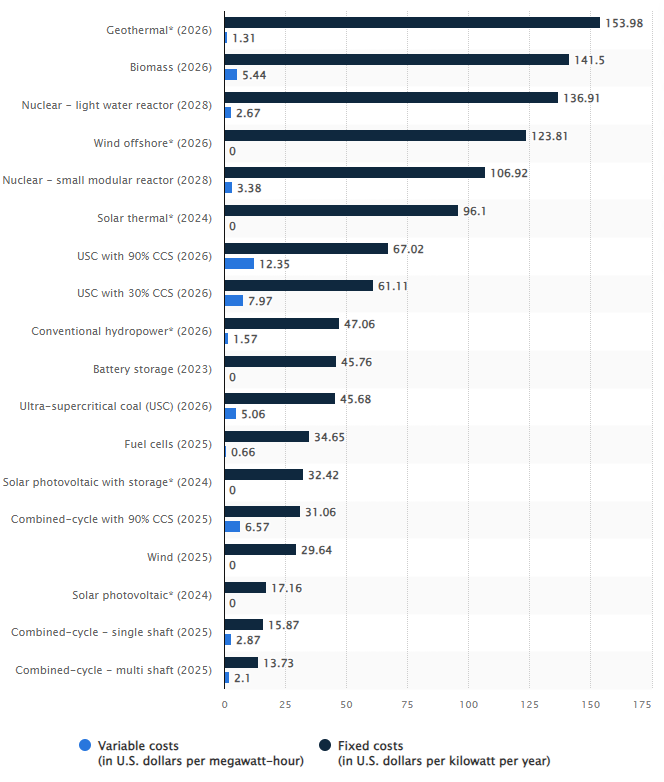
\includegraphics[scale=0.5]{StandardFigures/statista.png} 
\caption{Operations and Maintenance costs for various kinds of power plants.} 
\label{fig:statista} 
\end{figure} 

\begin{verbatim} 
C_OM = 60 * PE * 1000 = C700000  
\end{verbatim} 

Annualized O\&M costs are \$ C700000 M.

\subsubsection*{Cost Category 71 – O\&M Staff}
Component in the financial structuring of operational expenditures in various industries, especially those involving significant infrastructure and machinery, such as power generation, manufacturing, and utilities.  The costs under Cost Category 71 predominantly include:

\begin{itemize}
    \item \textbf{Salaries:} The regular wages paid to the O\&M staff.
    \item \textbf{Training and Development:} Costs associated with professional development, training programs, and certifications to ensure staff is up-to-date with the latest operational and maintenance practices.
    \item \textbf{Overtime and Shift Allowances:} Compensation for extended work hours and shift differentials, especially in 24/7 operational setups.
\end{itemize}

Cost Category 71 is crucial in operational budgeting due to:

\begin{enumerate}
    \item \textbf{Staffing Optimization:} The need for an optimal number of skilled staff to ensure efficient and safe operations.
    \item \textbf{Direct Impact on Operational Efficiency:} The performance and availability of O\&M staff directly affect operational uptime and efficiency.
    \item \textbf{Regulatory Compliance:} Compliance with labor laws and industry-specific regulations regarding staffing and worker safety.
\end{enumerate}

\textit{Cost Category 71 – O\&M Staff} encompasses all aspects of costs related to the personnel responsible for the operation and maintenance of facilities. Efficient management of this category is vital for ensuring operational excellence, staff well-being, and overall financial health of the organization.


\subsubsection*{Cost Category 72 – Management Staff}
Crucial aspect of operational expenses in various sectors, especially in industries where effective management plays a pivotal role in ensuring efficient operations and achieving organizational objectives.  Cost Category 72 typically encompasses:

\begin{itemize}
    \item \textbf{Salaries:} The basic remuneration paid to operations management staff.
    \item \textbf{Bonuses and Incentives:} Performance-related bonuses and incentives that align management objectives with corporate goals.
    \item \textbf{Professional Development:} Expenses related to the continuous learning and development of management skills, including workshops, seminars, and courses.
    \item \textbf{Leadership Training:} Specific training focused on enhancing leadership qualities necessary for effective management.
\end{itemize}

The inclusion of Cost Category 72 in operational expenditure is significant due to:

\begin{enumerate}
    \item \textbf{Strategic Decision Making:} Management staff play a crucial role in strategic decision-making and operational planning.
    \item \textbf{Operational Efficiency:} Effective management is key to ensuring operational efficiency and organizational success.
    \item \textbf{Staff Leadership:} Management staff are responsible for leading, guiding, and motivating the workforce, directly impacting productivity and morale.
\end{enumerate}

\textit{Cost Category 72 – Management Staff} is integral to the financial planning of any organization, particularly in operational contexts. It involves not just the direct costs of salaries and benefits but also the broader implications of effective management on organizational performance and success.

\subsubsection*{Cost Category 73 – Salary-Related Costs}
This Cost Category includes taxes, insurance, fringes, benefits, and any other annual salary-related costs.

\subsubsection*{Cost Category 74 – Operations Chemicals, and Lubricants}

\subsubsection*{Cost Category 75 – Spare Parts}
Critical element in the operational budgeting of various industries, particularly in sectors that rely on continuous and efficient machinery and equipment operation.  This cost category encompasses:

\begin{itemize}
    \item \textbf{Operational Spare Parts:} Expenses associated with spare parts used in regular operations. These do not include major equipment or capital plant upgrades.
    \item \textbf{Exclusion of Capitalized Items:} It specifically excludes items that would be capitalized or amortized over a period or quantity of product.
\end{itemize}

Cost Category 75 plays a significant role in Operations and Maintenance (O\&M) budgeting, as it:

\begin{itemize}
    \item \textbf{Ensures Operational Continuity:} Regular replacement and availability of spare parts are crucial for uninterrupted operations.
    \item \textbf{Impacts Maintenance Scheduling:} Influences the planning and scheduling of maintenance activities.
    \item \textbf{Affects Operational Efficiency:} Directly impacts the overall efficiency and lifespan of the operational equipment.
\end{itemize}

\textit{Cost Category 75 – Spare Parts} is essential for the smooth operation and maintenance of machinery and equipment in various industries. It encompasses the costs of spare parts necessary for regular operation and scheduled component replacements, playing a vital role in operational budgeting and efficiency.  Cost of any operational spare parts, excluding capital plant upgrades or major equipment that will be capitalized or amortized over some period or quantity of product.

\subsubsection*{Cost Category 76 – Utilities, Supplies, and Consumables}
Cost of water, gas, electricity, tools, machinery, maintenance equipment, office supplies and similar items purchased annually.

\subsubsection*{Cost Category 77 – Capital Plant Upgrades}
Upgrades to maintain or improve plant capacity, meet future regulatory requirements or plant life extensions.

\subsubsection*{Cost Category 78 – Taxes and Insurance}
Property taxes and insurance costs, excluding salary related.

\subsubsection*{Cost Category 79 – Contingency on Annualized O\&M Costs}
This Cost Category includes an assessment of additional cost necessary to achieve the desired confidence level for the annualized O\&M costs not to be exceeded.

\subsection{Cost Category 80: Annualized Fuel Cost (AFC)}

%\subsection{Annual Fuel Cost} 
The fuel cost, C$_{F}$, is calculated as follows.  The unit cost of deuterium as D2 is 3,700 \$/kg; deuterium contributes negligibly to the COE of a fusion power plant. In the long run, the power plant is self-sufficient in terms of tritium fuel production because of the breeding capability of the blanket so that no specific tritium-fuel charge is reported. It should be recognized, however, that there is a significant cost for tritium in the direct cost of the D-T fueled fusion reactor, represented in Cost Category 22.05 Fuel Handling and Storage. Cost of the primaryC and secondaryC coolant is included in Cost Category 27 Special Materials.\\

Consists of:  
\begin{verbatim} 
m_D = 3.342*10^(-27) # (kg)
u_D = 2175 #Where u_D ($/kg) = 2175 ($/kg) 
C_F = N_mod * P_NRL * 1e6 * 3600 * 8760 * u_D * m_D * p_a / (17.58 * 1.6021e-13)
\end{verbatim} 

Total annual fuel costs are \$ C800000 M per year.

\subsubsection*{Cost Category 81 – Refueling Operations}
This Cost Category includes incremental costs associated with refueling operations.

\subsubsection*{Cost Category 84 – Fuel}
This Cost Category includes annualized costs associated with the fuel cycle.

\subsubsection*{Cost Category 86 – Processing Charges}
This Cost Category includes storage and processing if fuel is brought in from offsite.

\subsubsection*{Cost Category 87 – Special Nuclear Materials}
This Cost Category covers materials such as heavy water, sodium, lead, helium, or other energy transfer mediums that are required on an annual basis. It includes costs associated with disposal or treatment if necessary. 

\subsubsection*{Cost Category 89 – Contingency on Annualized Fuel Costs}
This Cost Category includes an assessment of additional cost necessary to achieve the desired confidence level for the annualized fuel costs not to be exceeded.

\subsection{Cost Category 90: Annualized Financial Costs (AFC)}


Consists of: Capital recovery factor (or constant dollar FCR), $f_{cr}$ multiplied by the total capital cost. This is a function of the cost of money and the period over which the investment must be paid off (see 2019 NETL report \cite{NETL2019a}). In this case, it is the lifetime of the plant, plifetime years, plus the construction time, constructionTime years. Thus, the capital recovery factor is calculated from 

\begin{equation}
    C(x,N) = \frac{x(1+x)^N}{(1+x)^N-1} = \left[ \sum_{n=1}^N \frac{1}{(1+x)^N}] \right] ^{-1},
    \label{eq:C}
\end{equation}

where 

\begin{equation}
    x = i_cf_c + i_pf_p +(1-t)i_df_d
\end{equation}

is the effective cost of money. Here, $i_c$ is the rae of return on common stock, $f_c$ is the fraction of capital form common stock, $i_p$ is the rate of return of preferred stock, $f_p$ is the fraction of capital from preferred stock, $i_d$ is the nterest rate on deb, and $f_d$ is the capital from debt. 

From here, the fixed charge rate can be calculated as 
\begin{equation}
    f_{cr} = \frac{Ck}{(1-t)} - \frac{td}{(1-t)} + t_p + r,
\end{equation}

where $C$ is the capital recovery factor (\ref{eq:C}), $k$ is the adjustment for investment tax credit, $t$ is the effective income tax rate, $d$ is the levelized tax depreciation, $t_p$ is the property tax rate and $r$ is the levelized interim replacement cost. For this power plant, see \ref{tab:ec_vals} for values. Applying these calculations to this power plant with a lifetime of plifetime yields $f_{cr} = $ fcr.\\


\begin{table}
    \centering
    \begin{tabular}{cc|cc}
    \hline
      $N$ (plant life)  & plifetime & $t$ (construction period) & constructionTime\\
       $i_c$  & 0.1 & $t_p$ (property tax rate)& 0\\
        $i_p$ & 0 & $x_1$ (pre-tax)& 0.073\\
        $i_d$ & 0.05 & $x$ (post-tax)& 0.065\\
        $f_c$ & 0.45 & $x_r$ (real)& 0.045\\
        $f_p$ & 0 & $k$ & 1\\
        $f_d$ & 0.55 & $C(x,N)$ & 0.077\\
        $i$ (general inflation) & 0.02 & $C(x_r,N)$ & 0.061\\
        $e$  (escalation)& 0.02 & $r$ (interim replacement)& 0\\
        $e_r$ (real escalation) & 0 & $f$ (depreciable fraction of TCC)& 0.881\\
        $t_s$ (income tax 1) & 0.06 & $d$ (levelized depreciation)& 0.036\\
        $t_f$ (income tax 2) & 0.21 & $f_{cr}$ & 0.0910\\
        $t$ (effective income tax) & 0.257 & $f_{cr0}$ & 0.0722\\
    \hline    
    \end{tabular}
    \caption{Values used in calculation of capital recovery factor  $f_{cr}$, the effective cost of money, $x$, and the fixed charge rate, $R$.}
    \label{tab:ec_vals}
    \label{tab:my_label}
\end{table}

By multiplying the capital recovery factor, $f_{cr}$ by the total capital cost, $C_{99}$, the annual capital cost charge is calculated.
Annualized Financial Costs are \$ C900000 M.

\subsubsection*{Cost Category 91 – Escalation}
Critical financial concept often used in the planning and analysis of long-term projects, particularly in industries such as energy or construction. This category accounts for the changes in costs over time due to factors like inflation, market dynamics, and changes in labor or material costs. Escalation is the systematic increase in costs over the life of a project. It is distinct from \textit{contingency}, which is used to cover unforeseen costs. Escalation accounts for known, predictable changes in cost such as:

\begin{itemize}
    \item \textbf{Inflation:} General increase in prices and fall in the purchasing value of money.
    \item \textbf{Market Fluctuations:} Changes in costs due to supply and demand dynamics.
    \item \textbf{Labor Cost Changes:} Variations in labor costs due to economic conditions or labor market changes.
    \item \textbf{Material Cost Variations:} Fluctuations in the cost of raw materials.
\end{itemize}

In many financial estimates, particularly initial cost assessments, Cost Category 91 is often excluded. This exclusion is typically because:

\begin{enumerate}
    \item \textbf{Simplification:} To simplify the early stages of financial planning.
    \item \textbf{Variability:} Due to the unpredictable nature of some escalation factors.
\end{enumerate}

While often excluded from initial estimates, escalation is crucial in:

\begin{itemize}
    \item \textbf{Business Plans:} For a realistic long-term financial outlook.
    \item \textbf{Financing Proposals:} To present a complete picture to potential investors or lenders.
    \item \textbf{Regulatory-Related Documents:} Where detailed, realistic cost projections are required.
\end{itemize}

Effective management of Cost Category 91 involves:

\begin{enumerate}
    \item \textbf{Regular Reassessment:} Continuously updating the project's cost estimates to reflect current economic conditions.
    \item \textbf{Risk Mitigation:} Developing strategies to mitigate the impact of negative cost escalations.
    \item \textbf{Informed Decision Making:} Using escalation estimates to make informed financial and strategic decisions.
\end{enumerate}



\subsubsection*{Cost Category 92 – Fees}
This Cost Category primarily encompasses the costs associated with annual fees necessary for the operation of such facilities.  Fees under Cost Category 92 typically include, but are not limited to, costs related to:

\begin{itemize}
    \item \textbf{Licensed Reactor Processes:} These are fees paid for obtaining and maintaining the licenses required for reactor operation. They cover regulatory compliance and safety standards as set by nuclear regulatory bodies.
    \item \textbf{Nuclear Operating License Fees:} Fees associated with the acquisition and renewal of operating licenses for nuclear facilities. These are critical for legal and safe operation.
    \item \textbf{Regulatory Compliance:} Fees related to ensuring compliance with various environmental, safety, and operational regulations.
    \item \textbf{Inspection and Oversight:} Costs incurred for regular inspections and oversight activities by regulatory authorities to ensure adherence to safety and operational guidelines.
\end{itemize}

\textit{Cost Category 92 – Fees} is an essential financial Cost Category, especially for nuclear facilities, where regulatory compliance and licensing play a critical role. Proper management and allocation of funds for these fees are vital for uninterrupted and legal operation.

\subsubsection*{Cost Category 93 – Cost of Money}
The \textbf{cost of money} is akin to the \textit{opportunity cost} of using capital for a specific purpose. When capital is allocated to operating costs, it is an alternative to investing that capital elsewhere. Thus, the cost of money represents the return that this capital could have earned if invested differently.
\begin{itemize}
    \item Sources of Capital. Capital for operating costs can be sourced either externally or from within the organization (retained earnings). External financing includes loans, bonds, or other forms of borrowing, incurring interest payments. Retained earnings are internal funds saved and not distributed as dividends, carrying an opportunity cost as these funds could be used elsewhere.
    \item Impact on Operating Costs. In financial Cost Categorying, the cost of money is considered an \textit{indirect cost} of operating. It reflects the financial charges incurred due to the company's capital structure, including both the direct costs (e.g., interest on loans) and the opportunity costs (e.g., using retained earnings).
    \item Project Financing and Cost of Capital.  For large-scale projects like nuclear power plants, the cost of money is crucial in project financing. The strategy (debt vs. equity) and the corresponding costs of capital significantly affect the overall project economics.
    \item Risk and Return Considerations. The cost of money reflects the project's risk profile. Higher-risk projects lead to higher costs of capital, as lenders and investors demand higher returns for increased risks.
    \item Long-term Implications.  For long-term projects, the cost of money impacts the project's \textit{net present value} (NPV) and \textit{internal rate of return} (IRR). Effective management of the cost of money is essential for the project's long-term financial viability.
    \item Dynamic Nature.  The cost of money changes with market conditions, economic environment, and the organization's financial health. This necessitates continuous monitoring and reevaluation of financing strategies.
\end{itemize}

\textbf{In summary}, Cost Category 93 - Cost of Money - encompasses the financial implications of the capital used for operating costs. It includes both direct costs (like interest payments) and indirect costs (like opportunity costs of capital). Proper management of this Cost Category is crucial for the economic feasibility and financial health of large-scale projects.




\subsubsection*{Cost Category 99 – Contingency on Annualized Financial Costs}
This Cost Category includes an assessment of additional costs necessary to achieve the desired confidence level for the annualized financial costs not to be exceeded, including schedule uncertainties. Not included here.


\subsection{Levelized Cost of Electricity} 

\begin{table}[h!] 
\begin{tabular}{l c c } 
Net electric power & MW & PNET \\
Plant availability & \% & PAVAIL \\
Inflation & \% & INFL \\
Lifetime of plant & Years & Y \\
Capital cost, $C_{AC}$ &     M\$/annum    &    445      \\ 
Operations and Maintenance Costs, $C_{OM}$ & M\$/annum  &      4 \\ 
Fuel Costs, $C_{F}$ & M\$/annum  &       0 \\ 
    \end{tabular} 
    \caption{Cost components in the LCOE calcualtion.}
    \label{tab:lcoe} 
\end{table} 

Following equation \ref{eq:coe}, the LCOE is 947 \$/MWh or 95 c/kWh. 

%\subsection{Levelized Cost of Electricity Nth of a Kind (NOAK)}  

%It is possible to distinguish between the First of a Kind (FOAK) power plant, which might function as a Demo, and more mature 10th of a Kind (TOAK), the latter incorporating learning credits in the COE estimate, consistent with U.S. fusion-reactor design-community practice. The ARIES study, like STARFIRE \cite{BAK80} and most other U.S. fusion-reactor designs reported in the last decade, assumes FPC unit costs consistent with these learning-curve \cite{Hir64,Arg90} credits, rather than first-of-a-kind unit costs (including R\&D) appropriate for ITER \cite{Ite89} or some other reported designs \cite{Coo89b}. An 80 \% learning curve ({\it {\it i.e.},} 0.80 progress ratio, $p$), as used for ARIES, represents the expectation that each doubling of production represents a \hbox{$p\simeq$ 0.8} reduction in unit costs. A tenth-of-a-kind reactor represents, nominally, $\simeq$3.3 doubling of production or $p^{(ln 10/ln 2)}\simeq$ 50 \% cost reduction relative to first-of-a-kind FPC costs.  Of course, the actual production experience varies \cite{Arg90}.  Learning credits are not applied to BOP items, consistent with mature industrial production in which the learning credits have already been wrung out.  For similar reasons, a 94 \% learning curve is recommended for advanced fission cost estimates \cite{Del93}.   



\newpage 
  \appendix
  \newpage 
 \section{Glossary of terms} 
 \begin{description} 
 \item[ALPHA]{Accelerating Low-Cost Plasma Heating and Assembly} 
  \item[ARIES]{Advanced Reactor Innovation and Evaluation Study} 
  \item[ARPA-E]{Advanced Research Projects Agency - Energy} 
  \item[BOP]{ Balance of plant} 
  \item[CAD]{ Computer-aided design} 
  \item[CBS]{ Cost breakdown structure} 
  \item[DOE]{ U.S. Department of Energy} 
  \item[D-D]{ Deuterium-deuterium} 
  \item[D-T]{ Deuterium-tritium} 
  \item[ETS]{ Energy transfer and storage} 
  \item[FCR]{ Fixed charge rate} 
  \item[FPC]{ Fusion power core} 
  \item[FPP]{ Fusion power plant} 
  \item[FRC]{ Field reversed configuration} 
  \item[HP]{ High pressure} 
  \item[HVAC]{ Heating, ventilation, and air conditioning} 
  \item[I\&C]{ Instrumentation and control} 
  \item[IOU]{ Investor Owned Utility} 
  \item[IFE]{ Inertial fusion energy} 
  \item[kWh]{ Kilowatt Hour} 
  \item[LCOE]{ Levelized cost of electricity} 
  \item[LOCA]{ Loss of coolant accident} 
  \item[LP]{ Low pressure} 
  \item[MFE]{ Magnetic fusion energy} 
  \item[MIF]{ Magneto-inertial fusion} 
  \item[MTF]{ Magnetized target fusion} 
  \item[MW]{ Megawatt} 
  \item[MWe]{ Megawatt electric} 
  \item[MWth]{ Megawatt thermal} 
  \item[NEA]{ Nuclear Energy Agency} 
  \item[NIF]{ National Ignition Facility} 
  \item[NRL]{ Naval Research Laboratory} 
  \item[SLC]{ Stabilized liner compressor} 
  \item[SMR]{ Small modular reactor} 
  \item[TAE]{ TAE Technologies} 
  \item[USD]{ U.S. dollars} 
  \end{description} 
  \newpage 
\section{Bibliography} 
\bibliographystyle{IEEEtran.bst} 
\bibliography{ST-SC.bib,additions.bib}
\end{document} 
